% Appendix
\appendix
\section{Technical Specifications and Supplementary Details}
\label{sec:appendix}

This appendix provides detailed technical specifications, algorithmic implementations, and metric formulations that support the main text. Content is organized to facilitate reference while maintaining the narrative flow of the core contributions.

\subsection{Algorithm Specifications}
\label{app:algorithms}

This section details the algorithmic implementations of the distillation framework described in \autoref{sec:methodology}.

\subsubsection{Vocabulary Mapping Construction}
\label{app:vocab-mapping-alg}

Algorithm~\ref{alg:vocab-map-appendix} details the construction of the cross-vocabulary mapping $\psi: \mathcal{V} \to \mathcal{Z}$ from \autoref{def:vocab-mapping}.

\begin{algorithm}[H]
    \caption{BuildVocabularyMapping}
    \label{alg:vocab-map-appendix}
    \begin{algorithmic}
        \Require Road network $\mathcal{V}$ with centroid coordinates, Grid bounds and resolution
        \Ensure Mapping $\psi: \mathcal{V} \rightarrow \mathcal{Z}$
        \State Initialize $\psi \gets \{\}$
        \For{each road $r \in \mathcal{V}$}
        \State $(x_r, y_r) \gets \text{centroid}(r)$
        \State $i \gets \lfloor (x_r - x_{\min}) / \Delta_x \rfloor$ \Comment{Grid row index}
        \State $j \gets \lfloor (y_r - y_{\min}) / \Delta_y \rfloor$ \Comment{Grid column index}
        \State $z \gets i \cdot n_{\text{cols}} + j$ \Comment{Flatten to token ID}
        \State $\psi[r] \gets z$
        \EndFor
        \State \Return $\psi$
    \end{algorithmic}
\end{algorithm}

This deterministic mapping assigns each road segment's centroid to its containing grid cell, enabling cross-task knowledge transfer. Multiple roads may map to the same grid cell, particularly in dense urban areas.

\subsubsection{Distillation Loss Computation}
\label{app:distill-loss-alg}

Algorithm~\ref{alg:distill-loss-appendix} presents the forward KL divergence computation with gradient correction scaling from \autoref{thm:temp-scaling}.

\begin{algorithm}[H]
    \caption{ComputeDistillationLoss}
    \label{alg:distill-loss-appendix}
    \begin{algorithmic}
        \Require Teacher logits $\boldsymbol{\ell}^{\mathcal{L}}$, Student logits $\boldsymbol{\ell}^{\mathcal{H}}$, Candidates $\mathcal{C}_t$, Temperature $\tau$
        \Ensure Distillation loss $\mathcal{L}_{\text{KL}}^{(\tau)}$
        \State $q^{(\tau)} \gets \text{Softmax}(\boldsymbol{\ell}^{\mathcal{L}} / \tau)$ \Comment{Teacher distribution}
        \State $p^{(\tau)} \gets \text{Softmax}(\boldsymbol{\ell}^{\mathcal{H}} / \tau)$ \Comment{Student distribution}
        \State $\mathcal{L}_{\text{KL}} \gets 0$
        \For{each candidate $c \in \mathcal{C}_t$}
        \If{$q^{(\tau)}(c) > 0$} \Comment{Avoid $\log(0)$}
        \State $\mathcal{L}_{\text{KL}} \gets \mathcal{L}_{\text{KL}} + q^{(\tau)}(c) \cdot [\log q^{(\tau)}(c) - \log p^{(\tau)}(c)]$
        \EndIf
        \EndFor
        \State $\mathcal{L}_{\text{KL}}^{(\tau)} \gets \tau^2 \cdot \mathcal{L}_{\text{KL}}$ \Comment{Gradient correction}
        \State \Return $\mathcal{L}_{\text{KL}}^{(\tau)}$
    \end{algorithmic}
\end{algorithm}

The $\tau^2$ scaling factor ensures gradients remain well-scaled as temperature increases~\cite{hintonDistillingKnowledgeNeural2015}.


\subsubsection{Beam Search Generation}
\label{app:beam-search-alg}

Algorithm~\ref{alg:beam-search-appendix} details the trajectory generation procedure using beam search described in \autoref{sec:method-inference}.

\begin{algorithm}[H]
    \caption{BeamSearchGeneration}
    \label{alg:beam-search-appendix}
    \begin{algorithmic}
        \Require Origin $r_o$, Destination $r_d$, Student model $\mathcal{H}_{\theta^*}$, Beam width $b$
        \Ensure Generated trajectory $\hat{\mathbf{r}}$
        \State Initialize beams $\mathcal{B} \gets \{(r_o, 0.0)\}$ \Comment{(path, log-prob)}
        \State $t \gets 0$
        \While{$t < T_{\max}$ and no beam reached $r_d$}
        \State $\mathcal{B}_{\text{new}} \gets \{\}$
        \For{each $(path, score) \in \mathcal{B}$}
        \State $r_{\text{curr}} \gets \text{last}(path)$
        \State $\mathcal{C} \gets \text{GetCandidates}(r_{\text{curr}}, r_d)$ \Comment{Spatial pruning}
        \State $\boldsymbol{\ell} \gets \mathcal{H}_{\theta^*}(path, \mathcal{C})$ \Comment{Student inference}
        \State $\mathbf{p} \gets \text{Softmax}(\boldsymbol{\ell})$
        \For{each $c \in \text{top-}k(\mathbf{p}, b)$}
        \State $path' \gets path + [c]$
        \State $score' \gets score + \log p(c)$
        \State $\mathcal{B}_{\text{new}} \gets \mathcal{B}_{\text{new}} \cup \{(path', score')\}$
        \EndFor
        \EndFor
        \State $\mathcal{B} \gets \text{top-}b(\mathcal{B}_{\text{new}})$ by score
        \State $t \gets t + 1$
        \EndWhile
        \State \Return best complete path from $\mathcal{B}$
    \end{algorithmic}
\end{algorithm}

With beam width $b=4$, the student generates trajectories at $\sim$77 trajectories/second. Only the trained student $\mathcal{H}_{\theta^*}$ is used during inference---the teacher $\mathcal{L}_\phi$ is discarded after training.

\subsection{Evaluation Metrics}
\label{app:metrics}

This section provides detailed formulations for the evaluation metrics introduced in \autoref{sec:eval-metrics}.

\subsubsection{Global Distribution Metrics}
\label{app:global-metrics}

These metrics assess whether aggregate statistics of generated trajectories match real data distributions, regardless of individual trajectory alignment.

\paragraph{Jensen-Shannon Divergence (JSD)}

Symmetric divergence measure comparing probability distributions:

\begin{equation}
    \text{JSD}(P \parallel Q) = \frac{1}{2} D_{KL}(P \parallel M) + \frac{1}{2} D_{KL}(Q \parallel M)
    \label{eq:jsd-appendix}
\end{equation}

where $M = \frac{1}{2}(P + Q)$ is the mixture distribution and $D_{KL}(P \parallel Q) = \sum_i P(i) \log \frac{P(i)}{Q(i)}$ is the Kullback-Leibler divergence. JSD is bounded in $[0, 1]$, with 0 indicating identical distributions and 1 indicating completely disjoint distributions.

We compute JSD for three trajectory attributes, each requiring specific calculations and histogram binning:

\paragraph{Trip Distance Distribution}

For each trajectory (\autoref{def:trajectory}), we compute total trip distance using Haversine (great-circle) distance between consecutive road centroids:

\begin{equation}
    D(T) = \sum_{i=2}^{n} d_{\text{gc}}(\text{centroid}(r_{i-1}), \text{centroid}(r_i))
    \label{eq:trip-distance}
\end{equation}

where $d_{\text{gc}}(\cdot, \cdot)$ is the great-circle distance in kilometers. We create histograms with 100 bins spanning $[0, \max(\mathcal{D}_{\text{real}})]$ where $\mathcal{D}_{\text{real}}$ is the set of all real trajectory distances, plus one bin for $[\max(\mathcal{D}_{\text{real}}), \infty)$.

The Distance JSD is computed between normalized histograms:

\begin{equation}
    \text{JSD}_{\text{distance}} = \text{JSD}(H_{\text{real}}(\mathcal{D}) \parallel H_{\text{gen}}(\mathcal{D}))
    \label{eq:distance-jsd}
\end{equation}

where $H_{\text{real}}(\mathcal{D})$ and $H_{\text{gen}}(\mathcal{D})$ are the normalized histograms of real and generated trajectory distances.

\paragraph{Per-Segment Duration Distribution}

For timestamped trajectories (\autoref{def:trajectory-timestamped}), we extract \emph{per-segment} durations (not total trip duration):

\begin{equation}
    \Delta t_i = \frac{t_i - t_{i-1}}{60} \quad \text{for } i = 2, \ldots, n
    \label{eq:segment-duration}
\end{equation}

where durations are measured in minutes. Each segment contributes one sample to the duration distribution. Histograms use 100 bins spanning $[0, \max(\mathcal{T}_{\text{real}})]$ plus infinity bin.

The Duration JSD is computed between normalized histograms:

\begin{equation}
    \text{JSD}_{\text{duration}} = \text{JSD}(H_{\text{real}}(\mathcal{T}) \parallel H_{\text{gen}}(\mathcal{T}))
    \label{eq:duration-jsd}
\end{equation}

where $H_{\text{real}}(\mathcal{T})$ and $H_{\text{gen}}(\mathcal{T})$ are the normalized histograms of all segment durations from real and generated trajectories.

\paragraph{Radius of Gyration Distribution}

For each trajectory (\autoref{def:trajectory}), we calculate the radius of gyration as the \emph{mean distance} from trajectory points to their centroid (following the original HOSER evaluation implementation, not the RMS formula):

\begin{equation}
    R_g(T) = \frac{1}{|T|} \sum_{i=1}^{|T|} d_{\text{gc}}(\text{centroid}(r_i), \bar{c})
    \label{eq:radius-gyration}
\end{equation}

where $\bar{c} = (\bar{\text{lat}}, \bar{\text{lon}})$ is the geographic centroid of all road centroids in the trajectory:

\begin{equation}
    \bar{\text{lat}} = \frac{1}{|T|} \sum_{i=1}^{|T|} \text{lat}(\text{centroid}(r_i)), \quad
    \bar{\text{lon}} = \frac{1}{|T|} \sum_{i=1}^{|T|} \text{lon}(\text{centroid}(r_i))
    \label{eq:trajectory-centroid}
\end{equation}

Histograms use 100 bins spanning $[0, \max(\mathcal{R}_{\text{real}})]$ plus infinity bin.

The Radius of Gyration JSD is computed between normalized histograms:

\begin{equation}
    \text{JSD}_{\text{radius}} = \text{JSD}(H_{\text{real}}(\mathcal{R}) \parallel H_{\text{gen}}(\mathcal{R}))
    \label{eq:radius-jsd}
\end{equation}

where $H_{\text{real}}(\mathcal{R})$ and $H_{\text{gen}}(\mathcal{R})$ are the normalized histograms of radius of gyration values from real and generated trajectories. Lower JSD values indicate proper spatial complexity modeling.

\subsubsection{Local Trajectory Metrics}
\label{app:local-metrics}

These metrics compare individual trajectory pairs with matching OD endpoints, measuring point-by-point similarity.

\paragraph{Hausdorff Distance}

Maximum spatial deviation between two trajectories:

\begin{equation}
    H(A, B) = \max \left\{ \sup_{a \in A} \inf_{b \in B} d(a, b), \, \sup_{b \in B} \inf_{a \in A} d(a, b) \right\}
    \label{eq:hausdorff-appendix}
\end{equation}

where $A$ and $B$ are sets of trajectory points and $d(\cdot, \cdot)$ is Euclidean distance. This metric captures the worst-case spatial error between trajectories. Note: Hausdorff distance scales with trajectory length, so longer trajectories naturally have larger values.

\paragraph{Dynamic Time Warping (DTW)}

Cumulative distance under optimal temporal alignment:

\begin{equation}
    \text{DTW}(A, B) = \min_{\pi} \sum_{i=1}^{|\pi|} d(A[\pi_A(i)], B[\pi_B(i)])
    \label{eq:dtw-appendix}
\end{equation}

where $\pi = (\pi_A, \pi_B)$ is the warping path allowing non-linear time alignment, and $d(\cdot, \cdot)$ is Euclidean distance. DTW handles trajectories with different sampling rates or temporal variations but, like Hausdorff distance, also scales with trajectory length.

\paragraph{Edit Distance on Real Sequence (EDR)}

Normalized edit operations needed to transform one trajectory into another:

\begin{equation}
    \text{EDR}(A, B, \varepsilon) = \frac{\text{EditOps}(A, B, \varepsilon)}{\max(|A|, |B|)}
    \label{eq:edr-appendix}
\end{equation}

where $\text{EditOps}(A, B, \varepsilon)$ counts the minimum insertions, deletions, and substitutions needed to transform trajectory $A$ into $B$, with points within threshold $\varepsilon = 100$ meters considered matches. EDR is length-normalized ($\in [0,1]$) and robust to outliers, making it suitable for comparing trajectories of different lengths.

\subsubsection{Coverage Metrics}
\label{app:coverage-metrics}

\paragraph{OD Pair Matching Rate}

The percentage of generated trajectories whose \emph{actual endpoints} match real OD pairs in the dataset:

\begin{equation}
    \text{OD Match Rate} = \frac{|\{(o_{\text{gen}}, d_{\text{gen}}) \in \text{RealODs}\}|}{|\text{GeneratedTrajectories}|} \times 100\%
    \label{eq:od-match-appendix}
\end{equation}

\textbf{Critical distinction:} The model receives a target OD pair $(r_o, r_d)$ as input but may fail to reach $r_d$ during generation (e.g., getting stuck at intermediate road $r_i$). We extract the OD pair from the \emph{generated trajectory's actual endpoints} (first and last road ID), then check if this OD pair exists in real data using grid-based spatial binning (0.001° resolution, approximately 111m).

High matching rates indicate:
\begin{enumerate}[noitemsep,topsep=0pt]
    \item \textbf{Path completion success}: Model reaches intended destinations
    \item \textbf{Realistic OD patterns}: Generated endpoints align with real mobility patterns
\end{enumerate}

Low matching rates reveal fundamental navigation failures, even if other trajectory similarity metrics seem reasonable.

\subsection{Implementation Details}
\label{app:implementation}

\subsubsection{Hyperparameter Search Space}
\label{app:hyperparam-space}

Table~\ref{tab:hyperparam-search-appendix} details the complete hyperparameter search space for Optuna-based optimization described in \autoref{sec:impl-hparam}.

\begin{table}[H]
    \centering
    \caption{Hyperparameter search space and effects on knowledge distillation}
    \label{tab:hyperparam-search-appendix}
    \begin{tabular}{lll p{5.5cm}}
        \toprule
        \textbf{Parameter}         & \textbf{Range} & \textbf{Scale} & \textbf{Effect on Training}                                                                          \\
        \midrule
        $\lambda$ (distill weight) & [0.001, 0.1]   & Log            & Controls teacher influence vs. supervised signal. Higher values prioritize soft targets.             \\
        \addlinespace
        $\tau$ (temperature)       & [1.0, 5.0]     & Linear         & Smooths distributions; higher values expose more ``dark knowledge'' through relative probabilities.  \\
        \addlinespace
        $w$ (window size)          & [2, 8]         & Integer        & Teacher context length; larger windows provide more historical information but increase computation. \\
        \bottomrule
    \end{tabular}
\end{table}

The Optuna framework employs CMA-ES (Covariance Matrix Adaptation Evolution Strategy)~\cite{hansenCMAEvolutionStrategy2023} as the sampler for efficient continuous parameter space exploration, with Hyperband pruner~\cite{liHyperbandNovelBanditBased2018} terminating unpromising configurations early (minimum 5 epochs).

\subsubsection{Training Configuration}
\label{app:training-config}

Table~\ref{tab:training-config-appendix} provides complete training configuration ensuring fair comparison between vanilla and distilled models (referenced in \autoref{sec:eval-setup}).

\begin{table}[H]
    \centering
    \caption{Complete training configuration for fair model comparison}
    \label{tab:training-config-appendix}
    \begin{tabular}{lll}
        \toprule
        \textbf{Parameter}              & \textbf{Vanilla (Trial 0)}                                      & \textbf{Distilled (Optimal)}      \\
        \midrule
        Architecture                    & HOSER                                                           & HOSER (identical)                 \\
        Optimizer                       & AdamW ($\eta = 5 \times 10^{-4}$)                               & AdamW ($\eta = 5 \times 10^{-4}$) \\
        Weight decay                    & $1 \times 10^{-5}$                                              & $1 \times 10^{-5}$                \\
        Batch size                      & 128                                                             & 128                               \\
        Accumulation steps              & 8 (effective 1024)                                              & 8 (effective 1024)                \\
        Max epochs                      & 25                                                              & 25                                \\
        Learning rate schedule          & Cosine annealing                                                & Cosine annealing                  \\
        Warmup epochs                   & 2                                                               & 2                                 \\
        Data splits                     & Train/val/test                                                  & Train/val/test (identical)        \\
        Candidate top-$k$               & 64                                                              & 64                                \\
        Random seeds                    & 42, 43, 44                                                      & 42, 43, 44                        \\
        \midrule
        Distillation weight ($\lambda$) & 0 (disabled)                                                    & 0.0014                            \\
        Temperature ($\tau$)            & N/A                                                             & 4.37                              \\
        Teacher window ($w$)            & N/A                                                             & 7                                 \\
        \midrule
        \multicolumn{3}{l}{\textit{Hardware}}                                                                                                 \\
        \quad GPU                       & \multicolumn{2}{l}{NVIDIA RTX 2080 Ti (11GB VRAM)}                                                  \\
        \quad CPU                       & \multicolumn{2}{l}{Intel Xeon Silver 4216 @ 2.10GHz (16 cores)}                                     \\
        \quad RAM                       & \multicolumn{2}{l}{64GB DDR4}                                                                       \\
        \bottomrule
    \end{tabular}
\end{table}

This controlled experimental design ensures that performance differences stem purely from knowledge distillation, not confounding factors like different batch sizes, learning rates, or architectural choices.

\subsection{Dataset Specifications}
\label{app:datasets}

\subsubsection{Complete Dataset Statistics}
\label{app:dataset-stats}

Table~\ref{tab:dataset-stats-appendix} provides comprehensive statistics for all evaluation datasets (summary in \autoref{sec:data-overview}).

\begin{table}[H]
    \centering
    \caption{Complete trajectory dataset statistics and preprocessing details}
    \label{tab:dataset-stats-appendix}
    \small
    \begin{tabular}{lll}
        \toprule
        \textbf{Statistic}              & \textbf{Beijing}        & \textbf{Porto}        \\
        \midrule
        \multicolumn{3}{l}{\textit{Road Network}}                                    \\
        \quad Road segments             & 40,060                  & $\sim$11,024          \\
        \quad Spatial zones             & 300                     & 300                   \\
        \quad Grid cells (LM-TAD)       & 51,660 (205$\times$252) & 6,164 (46$\times$134) \\
        \midrule
        \multicolumn{3}{l}{\textit{Trajectories}}                                    \\
        \quad Training                  & 629,380                 & 481,359               \\
        \quad Validation                & 78,673                  & (see note)            \\
        \quad Test                      & 179,823                 & 137,532               \\
        \quad Total                     & 887,876                 & $\sim$700,000         \\
        \midrule
        \multicolumn{3}{l}{\textit{Trajectory Characteristics}}                      \\
        \quad Avg. length (roads)       & 4.6                     & 8.0                   \\
        \quad Avg. distance (km)        & 5.16                    & 3.66                  \\
        \quad Avg. duration (min)       & 28.2                    & 12.3                  \\
        \quad Max length (roads)        & 1024 (truncated)        & 1024 (truncated)      \\
        \midrule
        \multicolumn{3}{l}{\textit{Preprocessing}}                                   \\
        \quad Map-matching quality      & High (HOSER authors)    & High (HOSER authors)  \\
        \quad Partition time (sec)      & 15--20                  & 4                     \\
        \quad Zone trans. matrix (sec)  & 10--15                  & 67                    \\
        \quad Vocab. mapping time (sec) & $<$1                    & $<$1                  \\
        \midrule
        \multicolumn{3}{l}{\textit{Data Splits}}                                     \\
        \quad Split strategy            & OD-stratified           & OD-stratified         \\
        \quad Test OD overlap           & 0\% (held-out)          & 0\% (held-out)        \\
        \bottomrule
    \end{tabular}
\end{table}

\textbf{Note on trajectory length:} Porto trajectories are substantially longer than Beijing (8.0 vs 4.6 road segments on average), leading to quadratic memory scaling in attention mechanisms. This necessitates reduced batch sizes for Porto experiments (see \autoref{sec:impl-practical}).

\textbf{Note on Porto validation set:} Porto validation split size is not explicitly documented in available evaluation reports. The dataset uses OD-stratified train/test splits with 481,359 training and 137,532 test trajectories. Validation split methodology follows the HOSER framework but specific counts are pending verification from source data.

\subsubsection{Vocabulary Alignment Details}
\label{app:vocab-stats}

Table~\ref{tab:vocab-alignment-appendix} summarizes vocabulary alignment characteristics between HOSER roads and LM-TAD grid cells (introduced in \autoref{sec:data-lmtad-compat}).

\begin{table}[H]
    \centering
    \caption{Vocabulary alignment between HOSER roads and LM-TAD grid cells}
    \label{tab:vocab-alignment-appendix}
    \begin{tabular}{lcccc}
        \toprule
        \textbf{Dataset} & \textbf{Roads ($|\mathcal{V}|$)} & \textbf{Grid Size} & \textbf{Cells ($|Z|$)} & \textbf{Avg. Roads/Cell} \\
        \midrule
        Beijing          & 40,060                           & 205 $\times$ 252   & 51,660                 & 0.78                     \\
        Porto            & 11,024                           & 46 $\times$ 134    & 6,164                  & 1.79                     \\
        \bottomrule
    \end{tabular}
\end{table}

The many-to-one mapping (multiple roads per grid cell) is inevitable in dense urban areas. Grid resolution is chosen to balance spatial granularity (finer grids capture local patterns) with vocabulary size (larger vocabularies increase computational cost).

\subsection{Supplementary Figures}
\label{app:figures}

This section provides comprehensive visual documentation of hyperparameter optimization, distribution analyses, trajectory examples, and cross-model comparisons that support the evaluation presented in \autoref{sec:evaluation}.

\subsubsection{Hyperparameter Optimization (Porto)}
\label{app:optuna-porto}

Figure~\ref{fig:appendix-optuna-phase1} and Figure~\ref{fig:appendix-optuna-phase2} present additional Optuna visualization plots for Porto Phase 1 and Phase 2 hyperparameter optimization, complementing the optimization history and parameter importance plots shown in \autoref{sec:impl-hparams}.

\begin{figure}[H]
    \centering
    \begin{subfigure}{0.49\linewidth}
        \centering
        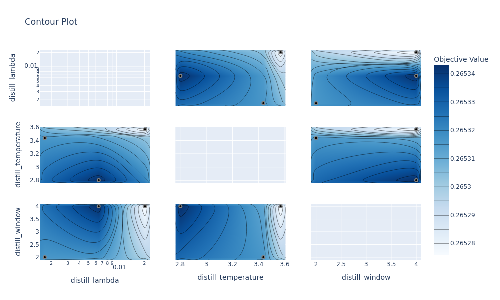
\includegraphics[width=\linewidth]{assets/plots/eval/porto/optuna/phase1/contour_plot.pdf}
        \caption{Parameter contour plot}
    \end{subfigure}
    \begin{subfigure}{0.49\linewidth}
        \centering
        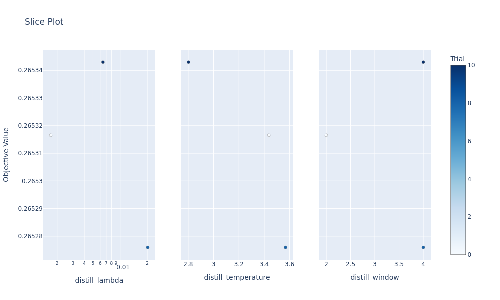
\includegraphics[width=\linewidth]{assets/plots/eval/porto/optuna/phase1/slice_plot.pdf}
        \caption{Parameter slice plot}
    \end{subfigure}
    \begin{subfigure}{0.49\linewidth}
        \centering
        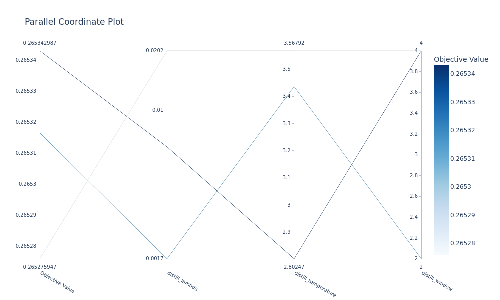
\includegraphics[width=\linewidth]{assets/plots/eval/porto/optuna/phase1/parallel_coordinate.pdf}
        \caption{Parallel coordinate plot}
    \end{subfigure}
    \caption{Porto Phase 1 hyperparameter optimization analysis. Contour and slice plots reveal parameter interactions and sensitivities. Parallel coordinates show trial progression through the search space.}
    \label{fig:appendix-optuna-phase1}
\end{figure}

\begin{figure}[H]
    \centering
    \begin{subfigure}{0.49\linewidth}
        \centering
        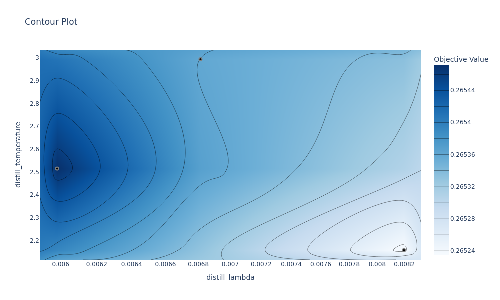
\includegraphics[width=\linewidth]{assets/plots/eval/porto/optuna/phase2/contour_plot.pdf}
        \caption{Parameter contour plot}
    \end{subfigure}
    \begin{subfigure}{0.49\linewidth}
        \centering
        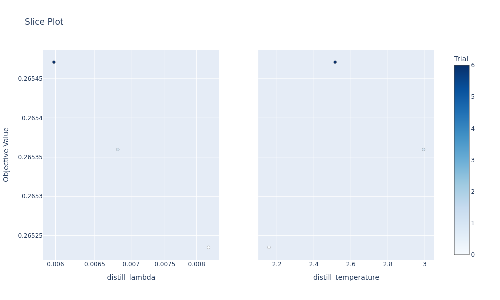
\includegraphics[width=\linewidth]{assets/plots/eval/porto/optuna/phase2/slice_plot.pdf}
        \caption{Parameter slice plot}
    \end{subfigure}
    \begin{subfigure}{0.49\linewidth}
        \centering
        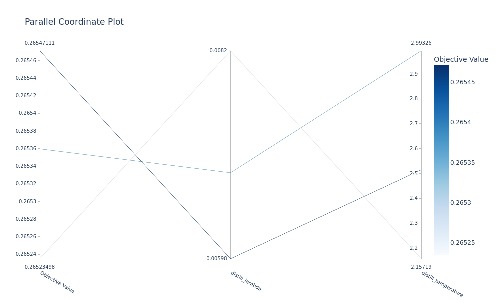
\includegraphics[width=\linewidth]{assets/plots/eval/porto/optuna/phase2/parallel_coordinate.pdf}
        \caption{Parallel coordinate plot}
    \end{subfigure}
    \caption{Porto Phase 2 hyperparameter optimization analysis. Refinement phase shows tighter parameter distributions and more consistent trial performance compared to Phase 1.}
    \label{fig:appendix-optuna-phase2}
\end{figure}

\subsubsection{Scenario-Level Analysis (Beijing)}
\label{app:scenario-beijing}

Figures~\ref{fig:appendix-beijing-scenario-heatmap} through~\ref{fig:appendix-beijing-scenario-spatial} present scenario-level performance breakdowns for Beijing, supporting the context-dependent analysis in \autoref{sec:eval-beijing}.

\begin{figure}[H]
    \centering
    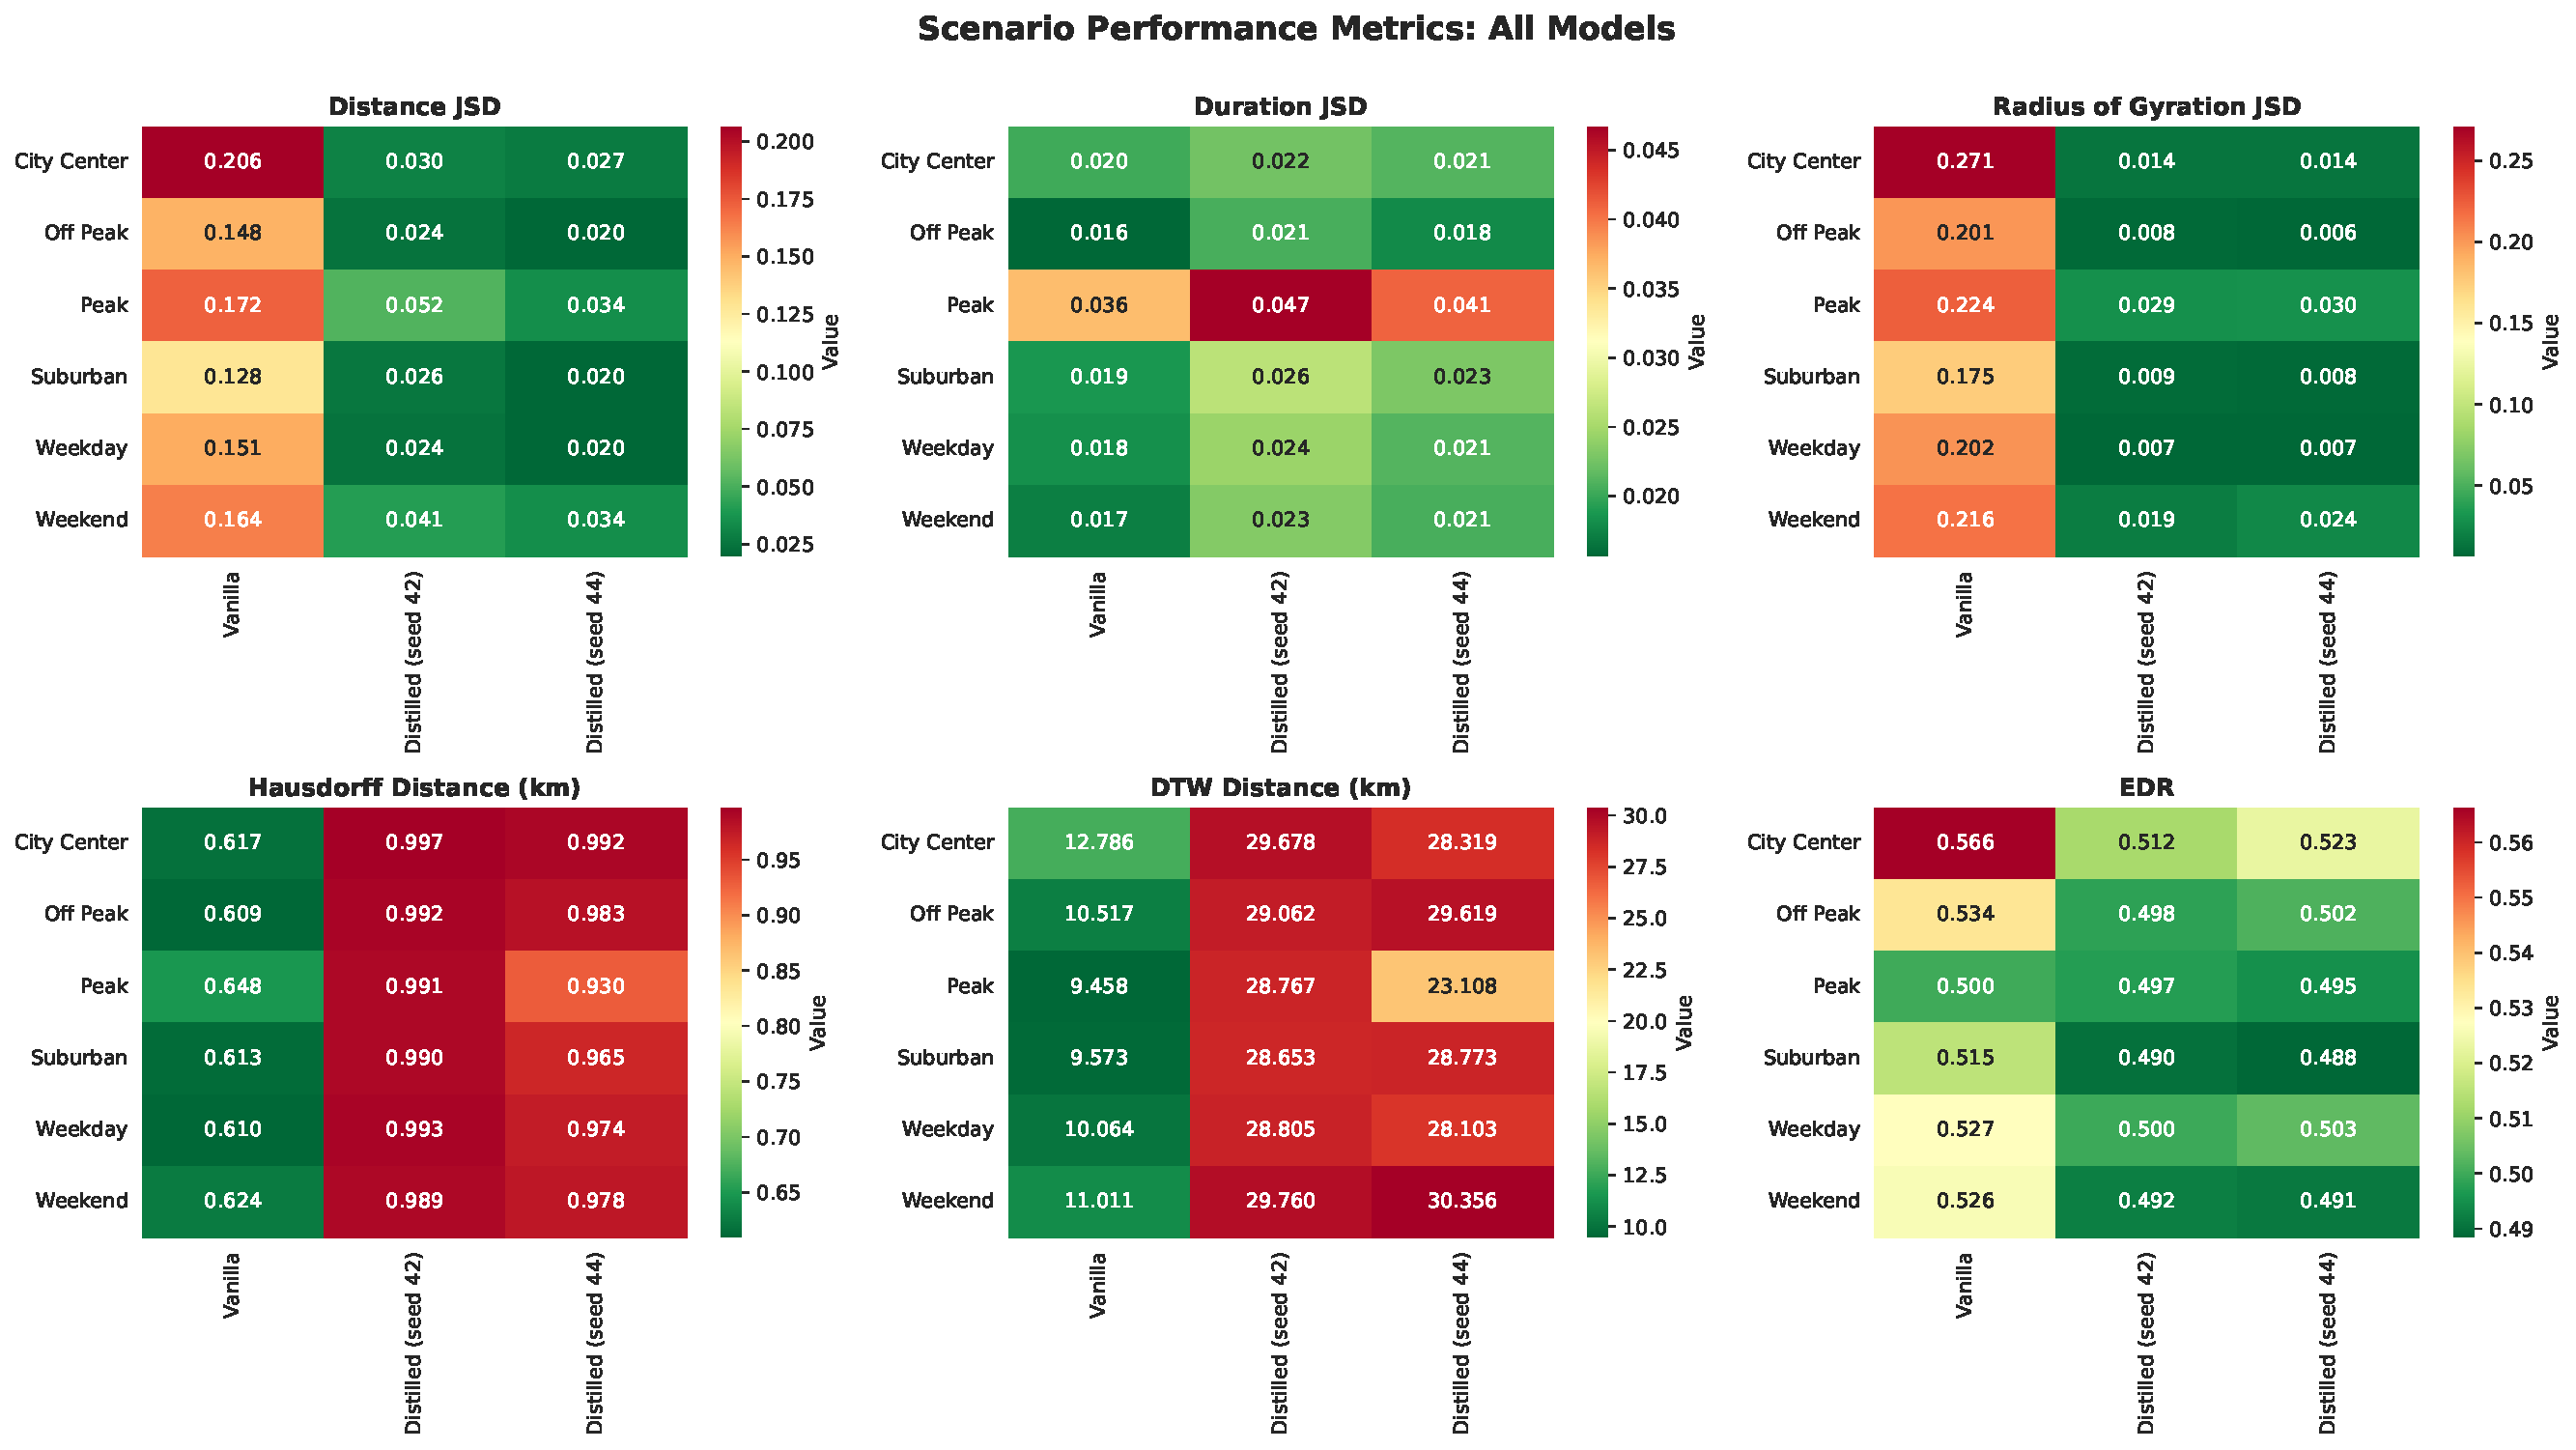
\includegraphics[width=0.85\linewidth]{assets/plots/eval/beijing/scenarios/scenario_metrics_heatmap.pdf}
    \caption{Beijing scenario-level metrics heatmap showing performance across spatial and temporal contexts. Distilled models maintain consistent high performance across all scenarios.}
    \label{fig:appendix-beijing-scenario-heatmap}
\end{figure}

\begin{figure}[H]
    \centering
    \begin{subfigure}{0.49\linewidth}
        \centering
        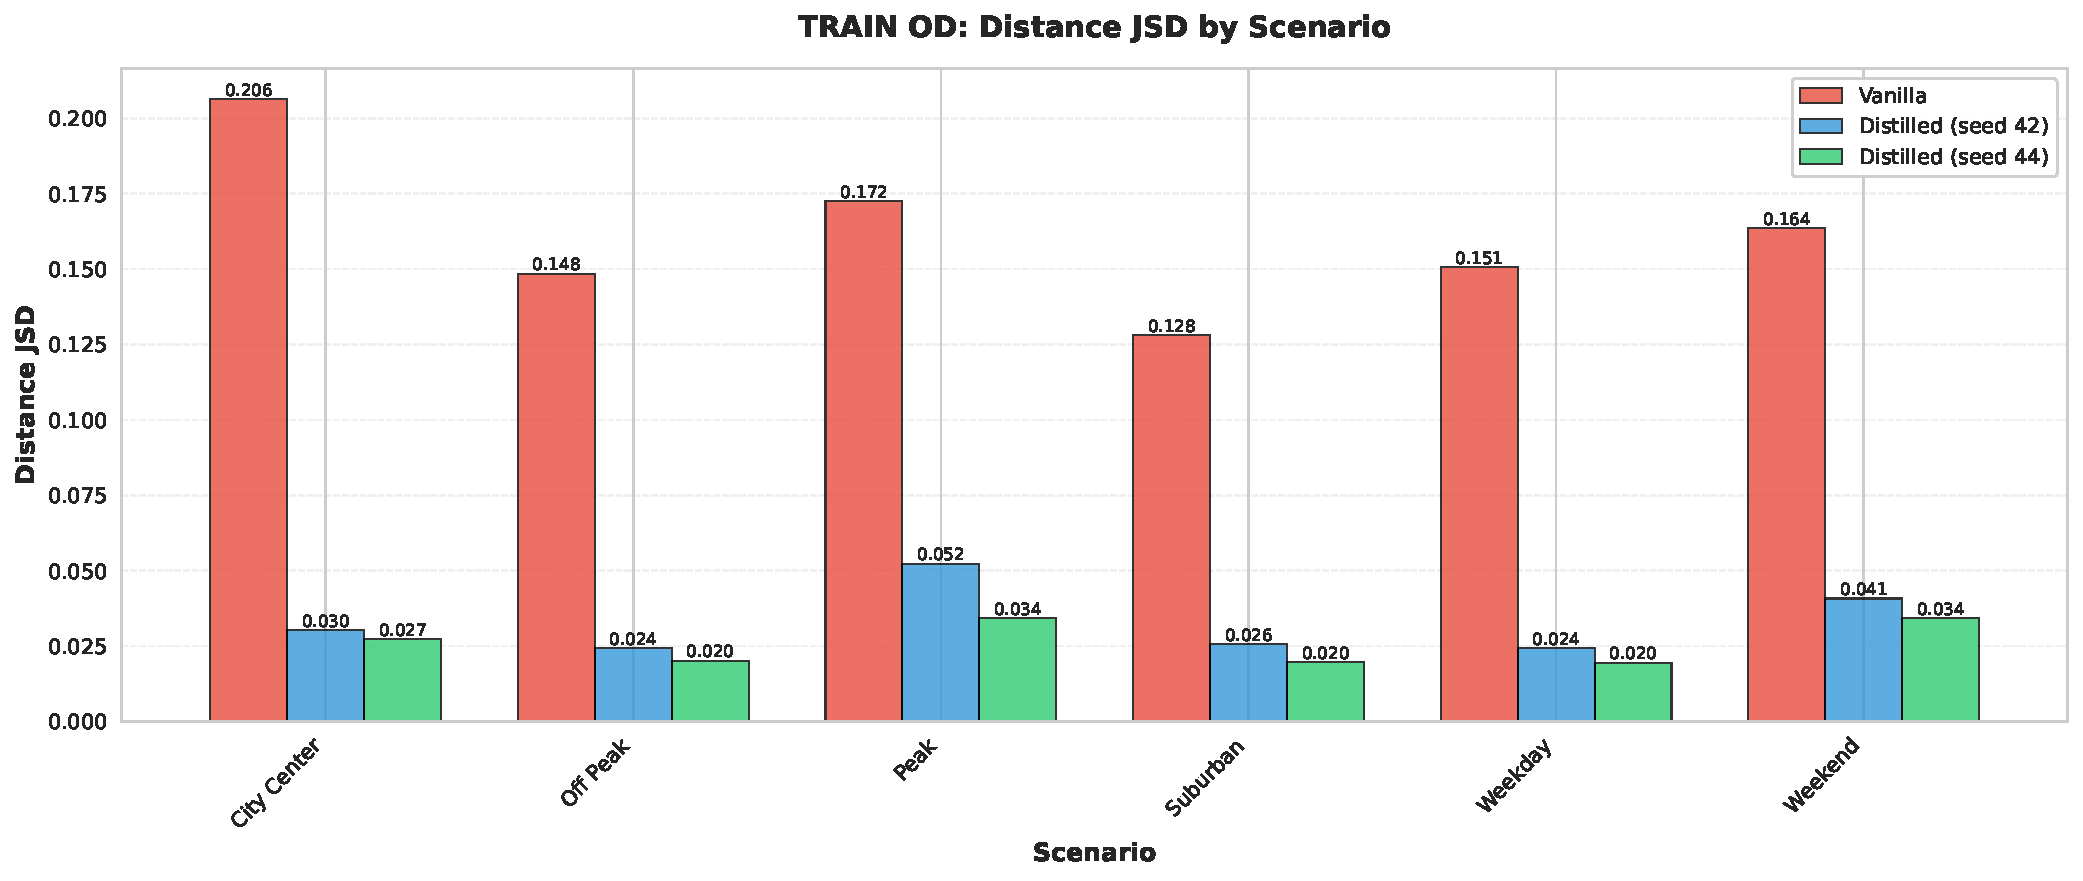
\includegraphics[width=\linewidth]{assets/plots/eval/beijing/scenarios/train_od_scenario_comparison.pdf}
        \caption{Train OD scenarios}
    \end{subfigure}
    \begin{subfigure}{0.49\linewidth}
        \centering
        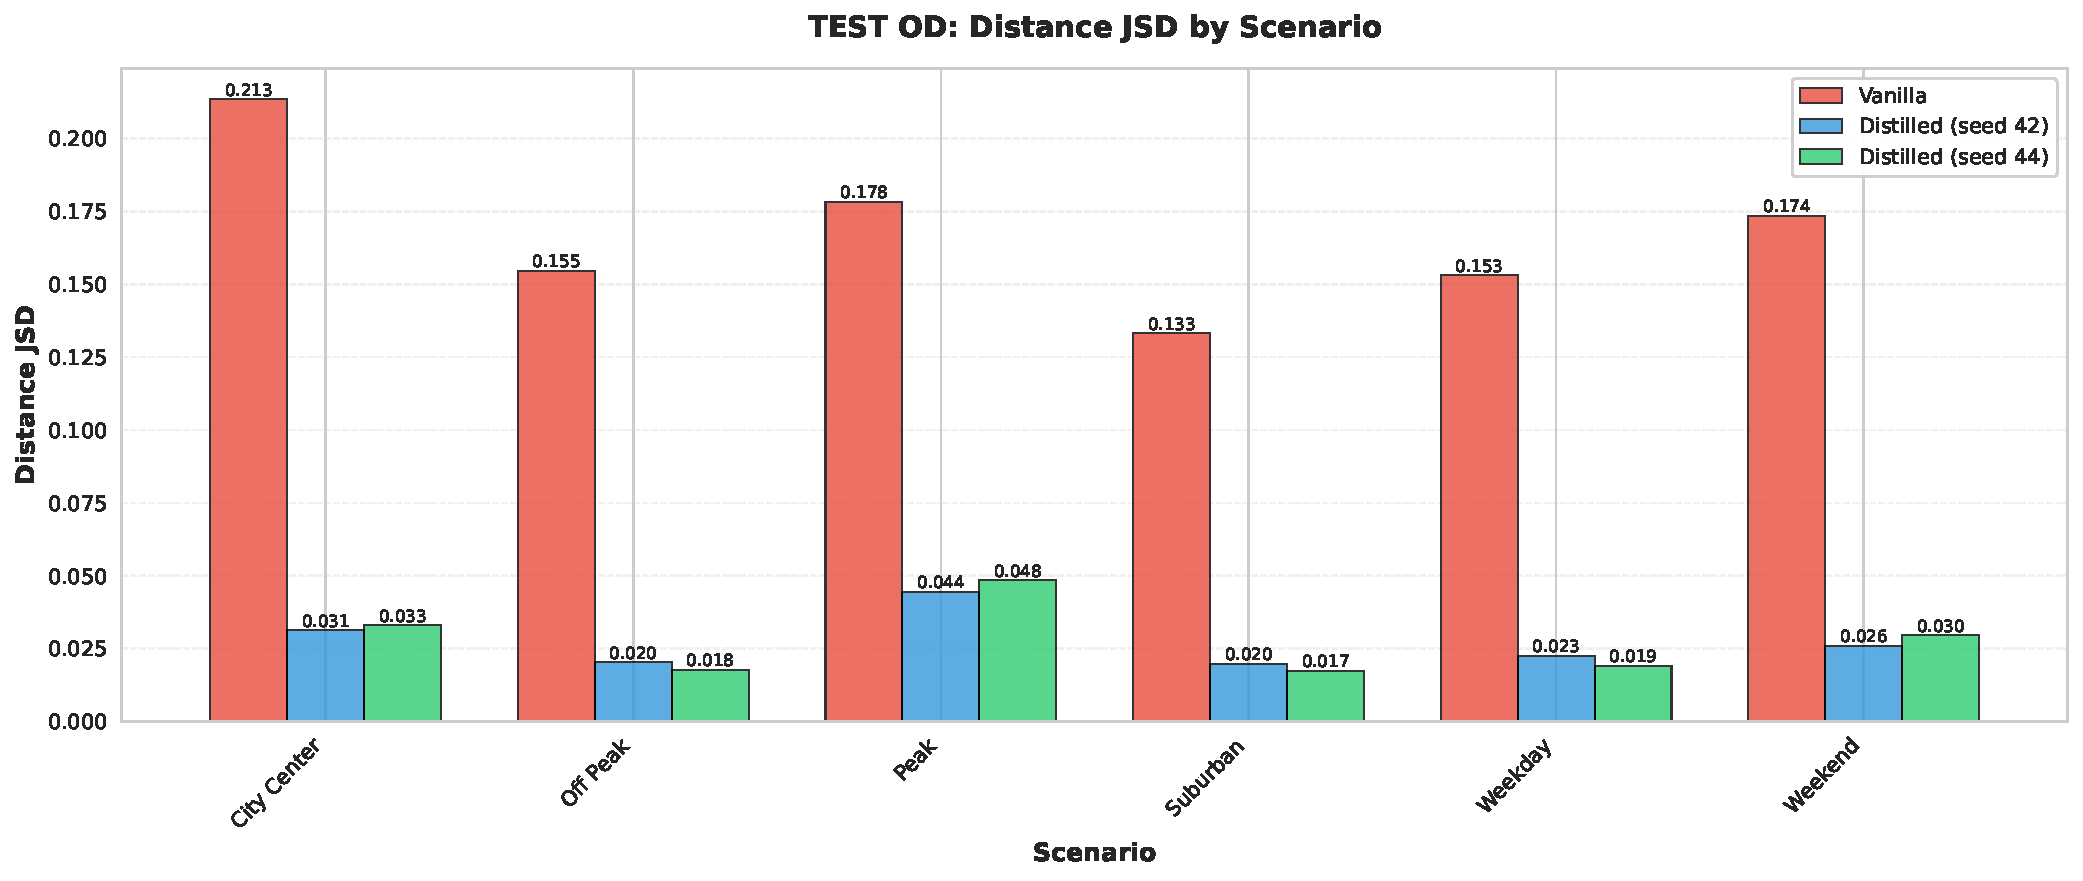
\includegraphics[width=\linewidth]{assets/plots/eval/beijing/scenarios/test_od_scenario_comparison.pdf}
        \caption{Test OD scenarios}
    \end{subfigure}
    \caption{Beijing scenario comparison across train and test OD pairs. Distilled models show consistent superiority regardless of spatial or temporal context.}
    \label{fig:appendix-beijing-scenario-comparison}
\end{figure}

\begin{figure}[H]
    \centering
    \begin{subfigure}{0.49\linewidth}
        \centering
        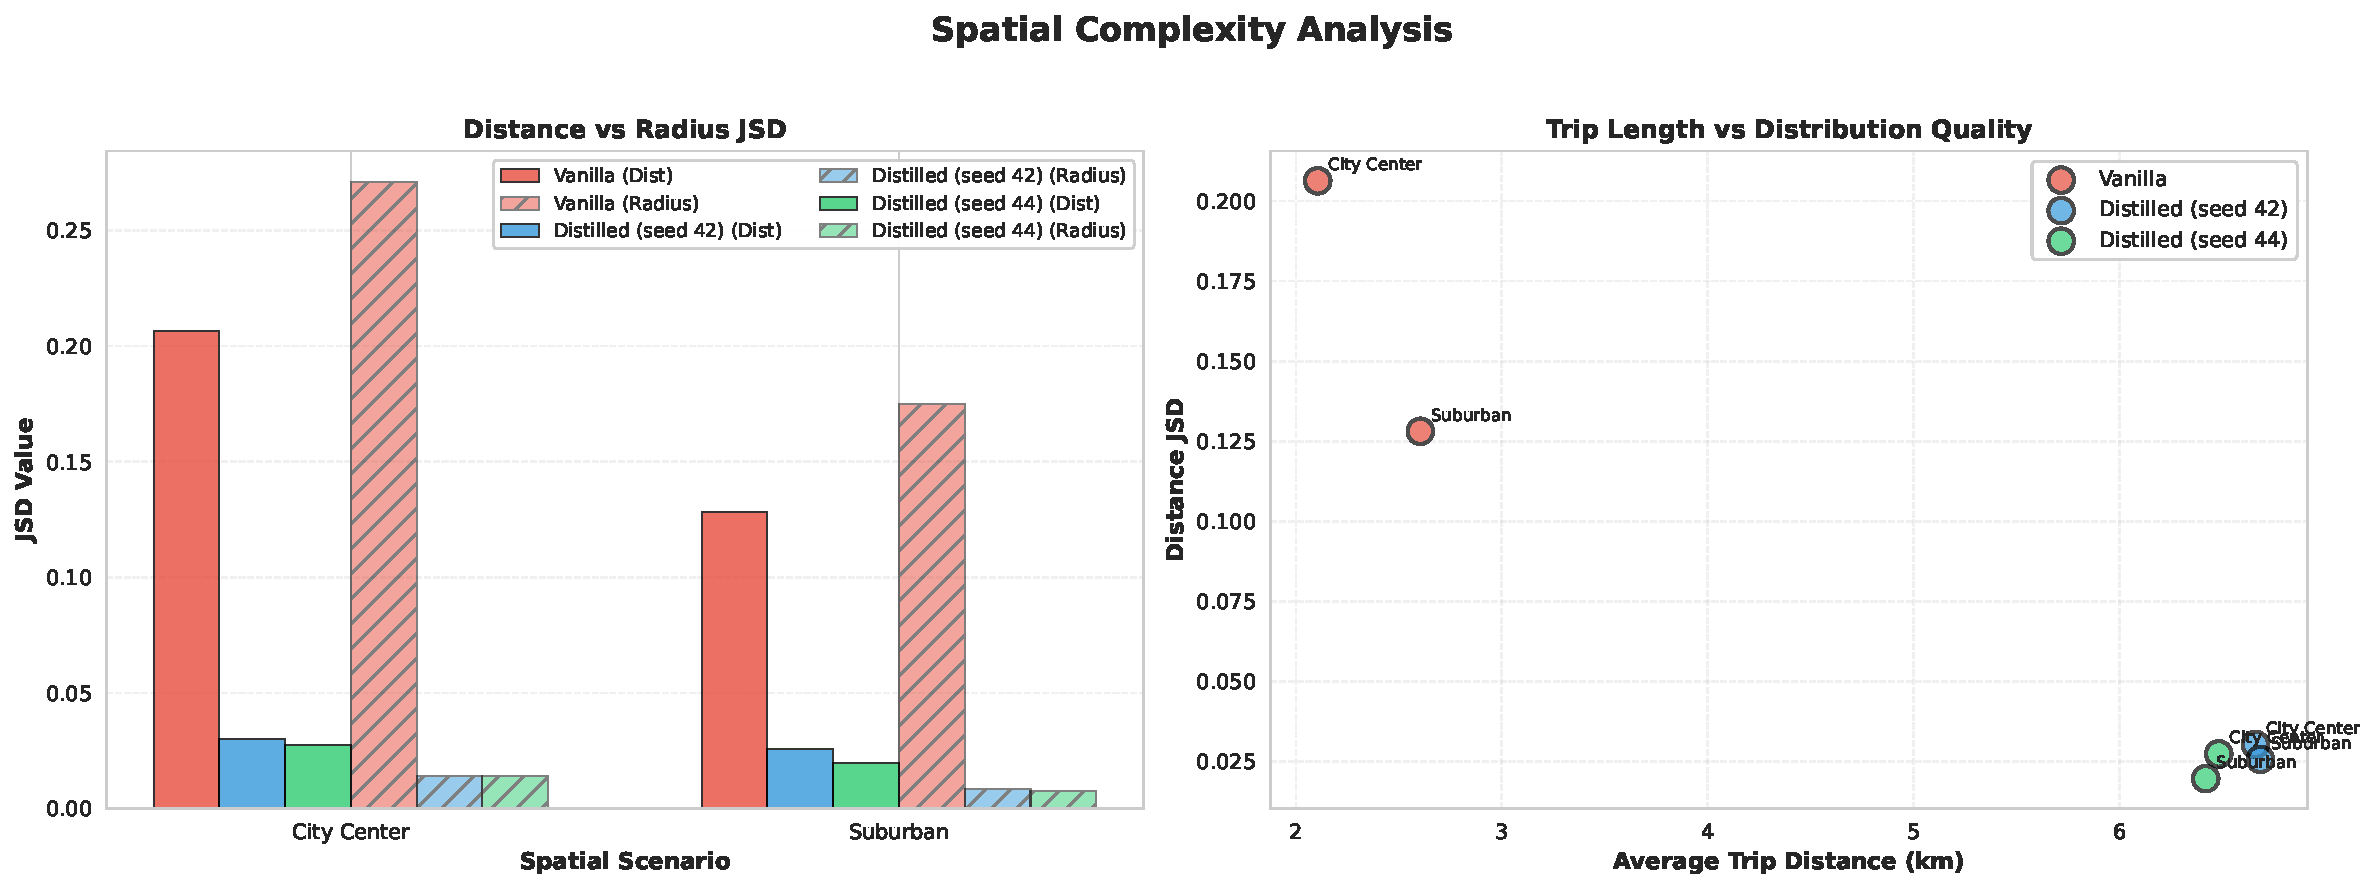
\includegraphics[width=\linewidth]{assets/plots/eval/beijing/scenarios/spatial_scenarios_analysis.pdf}
        \caption{Spatial context analysis}
    \end{subfigure}
    \begin{subfigure}{0.49\linewidth}
        \centering
        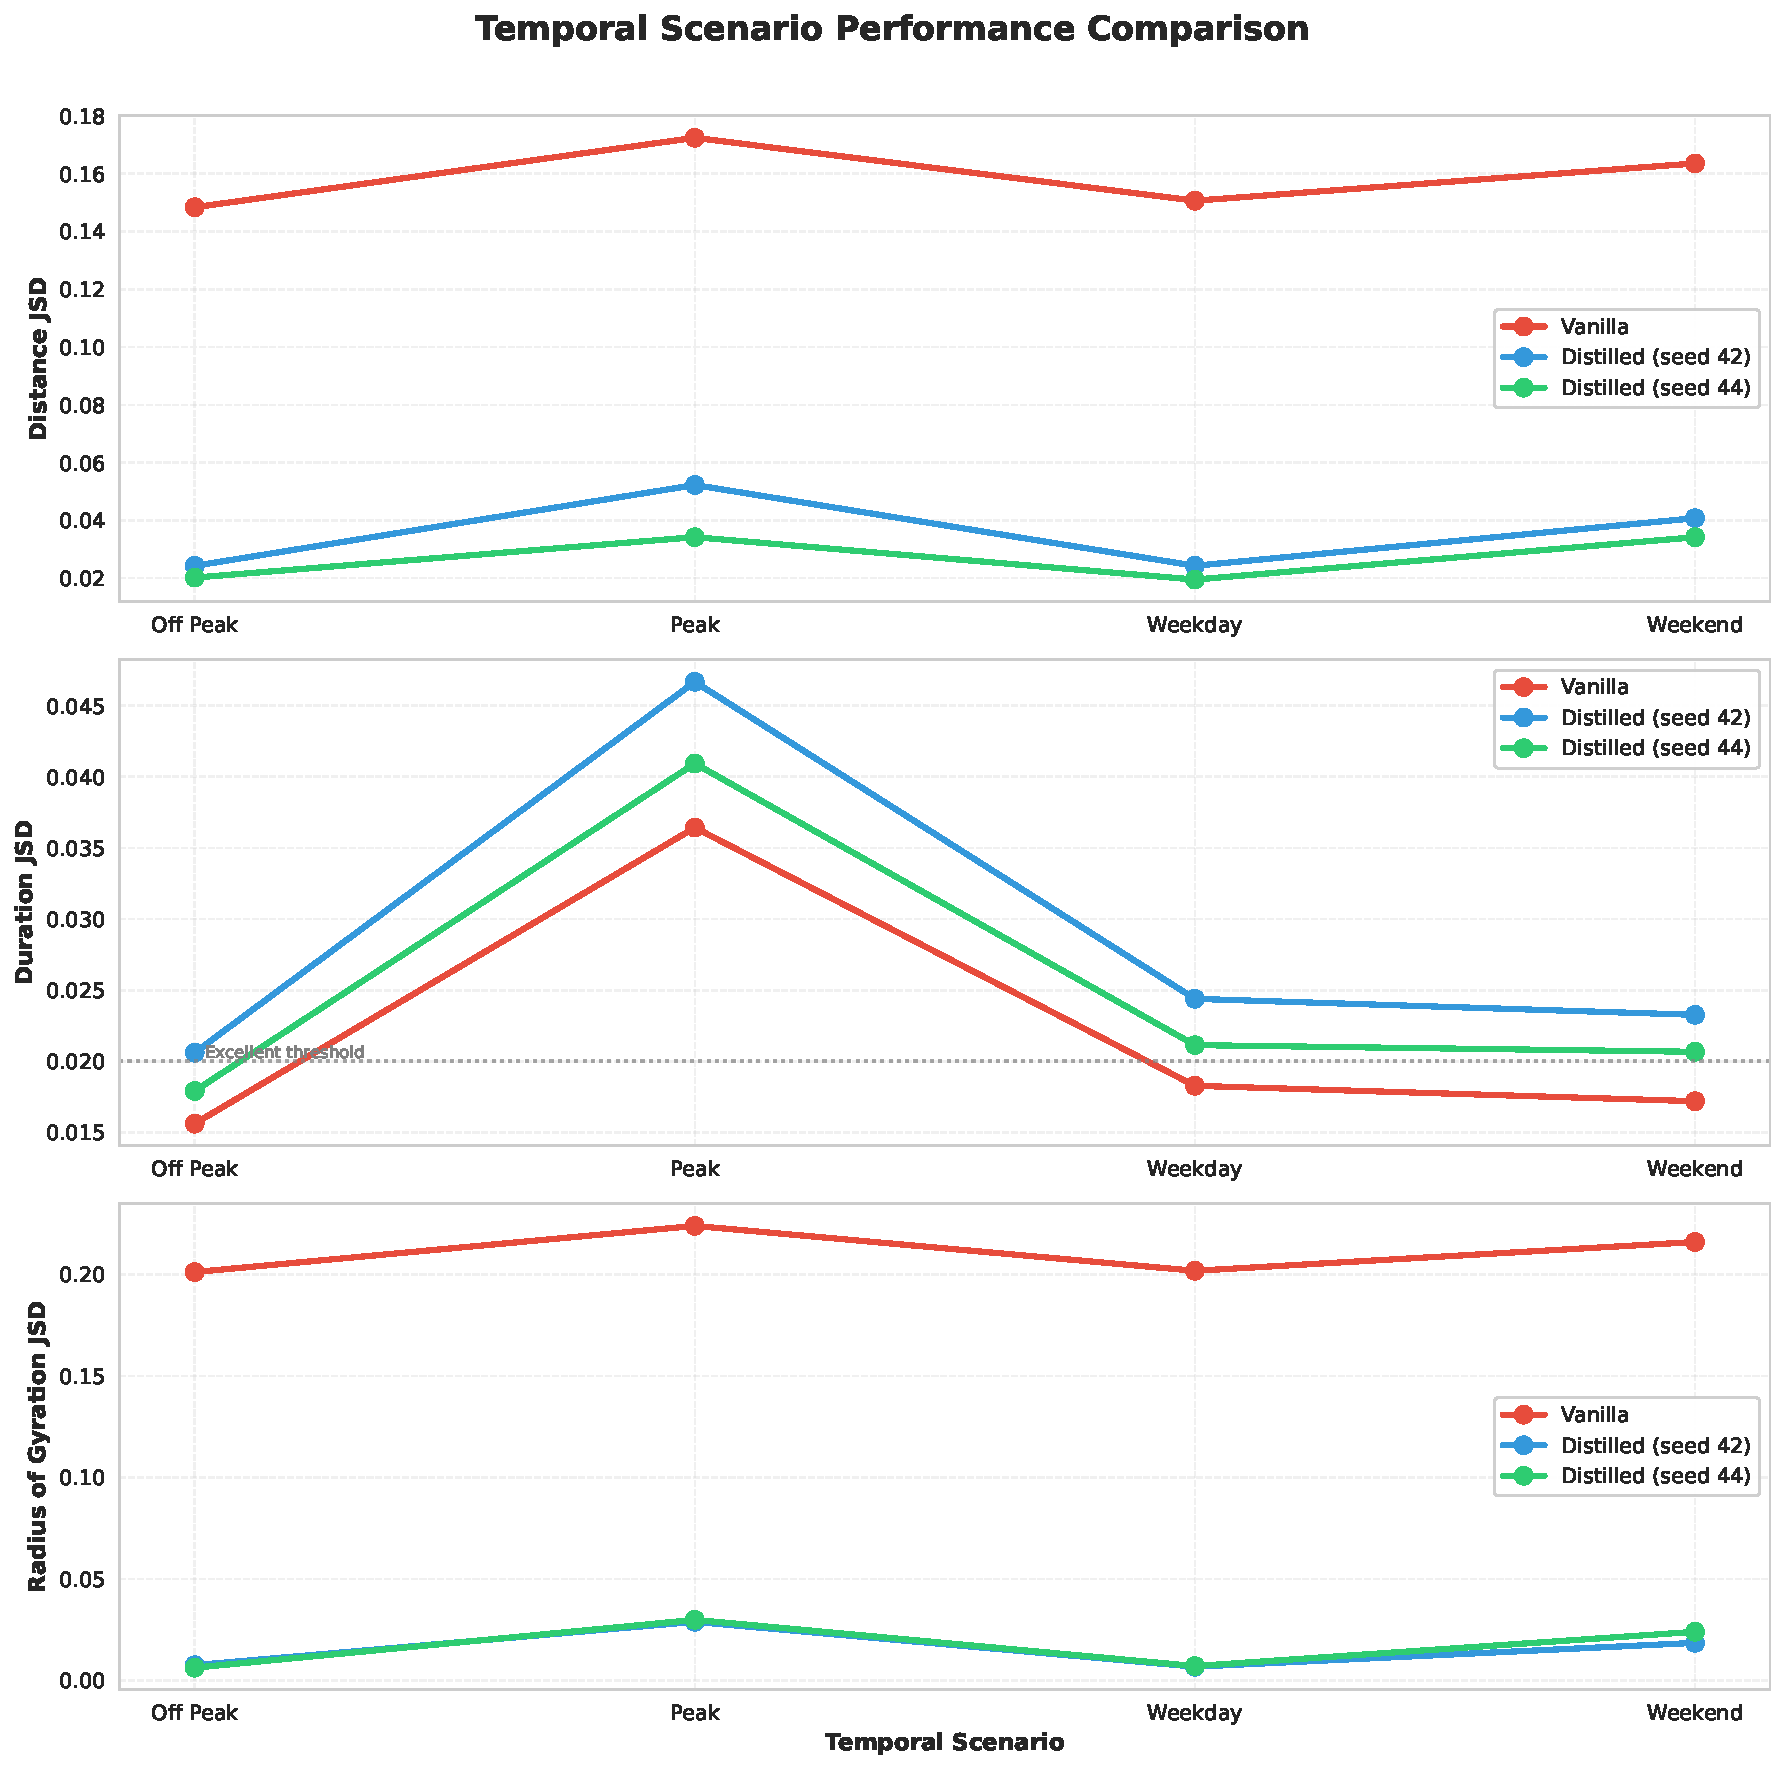
\includegraphics[width=\linewidth]{assets/plots/eval/beijing/scenarios/temporal_scenarios_comparison.pdf}
        \caption{Temporal context analysis}
    \end{subfigure}
    \caption{Beijing spatial and temporal scenario performance. Universal improvement across all contexts demonstrates robust knowledge transfer.}
    \label{fig:appendix-beijing-scenario-spatial}
\end{figure}

\subsubsection{Scenario-Level Analysis (Porto)}
\label{app:scenario-porto}

Figures~\ref{fig:appendix-porto-scenario-heatmap} through~\ref{fig:appendix-porto-scenario-sensitivity} present scenario-level performance breakdowns for Porto, revealing context-dependent behavior discussed in \autoref{sec:eval-porto}.

\begin{figure}[H]
    \centering
    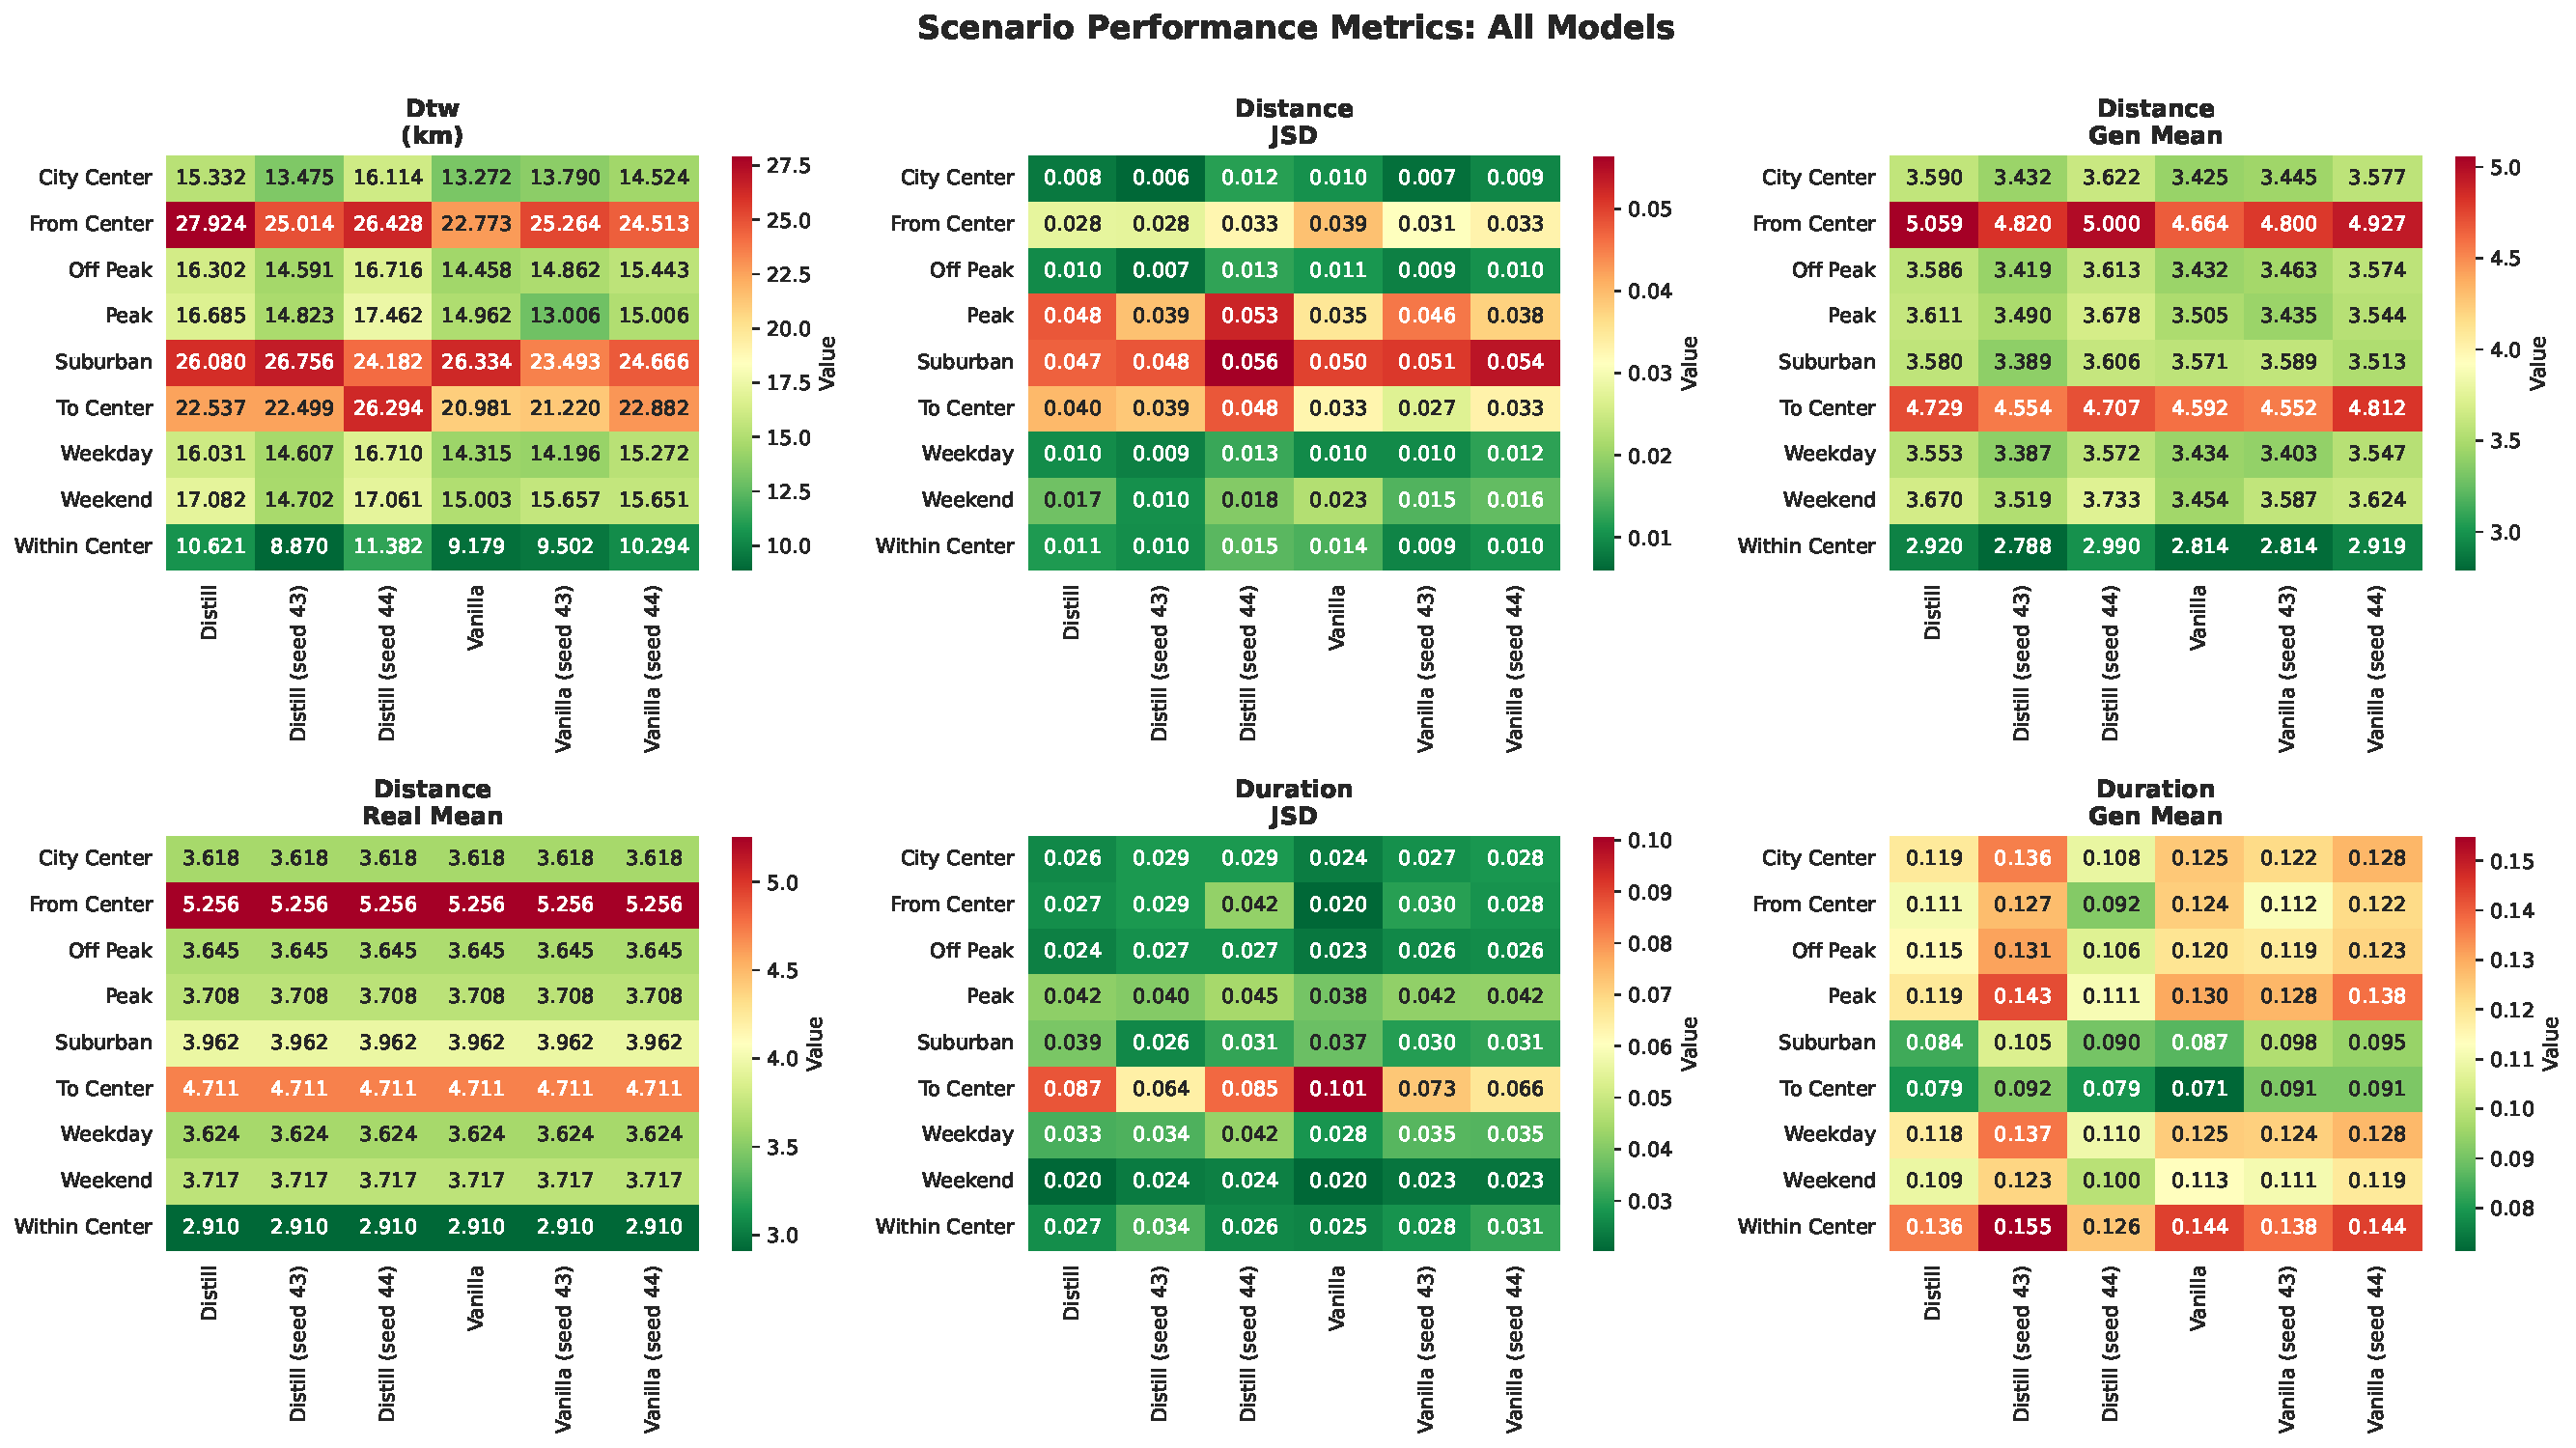
\includegraphics[width=0.85\linewidth]{assets/plots/eval/porto/scenarios/scenario_metrics_heatmap.pdf}
    \caption{Porto scenario-level metrics heatmap showing spatially localized performance gains. Distillation benefits concentrate in suburban and rural contexts.}
    \label{fig:appendix-porto-scenario-heatmap}
\end{figure}

\begin{figure}[H]
    \centering
    \begin{subfigure}{0.49\linewidth}
        \centering
        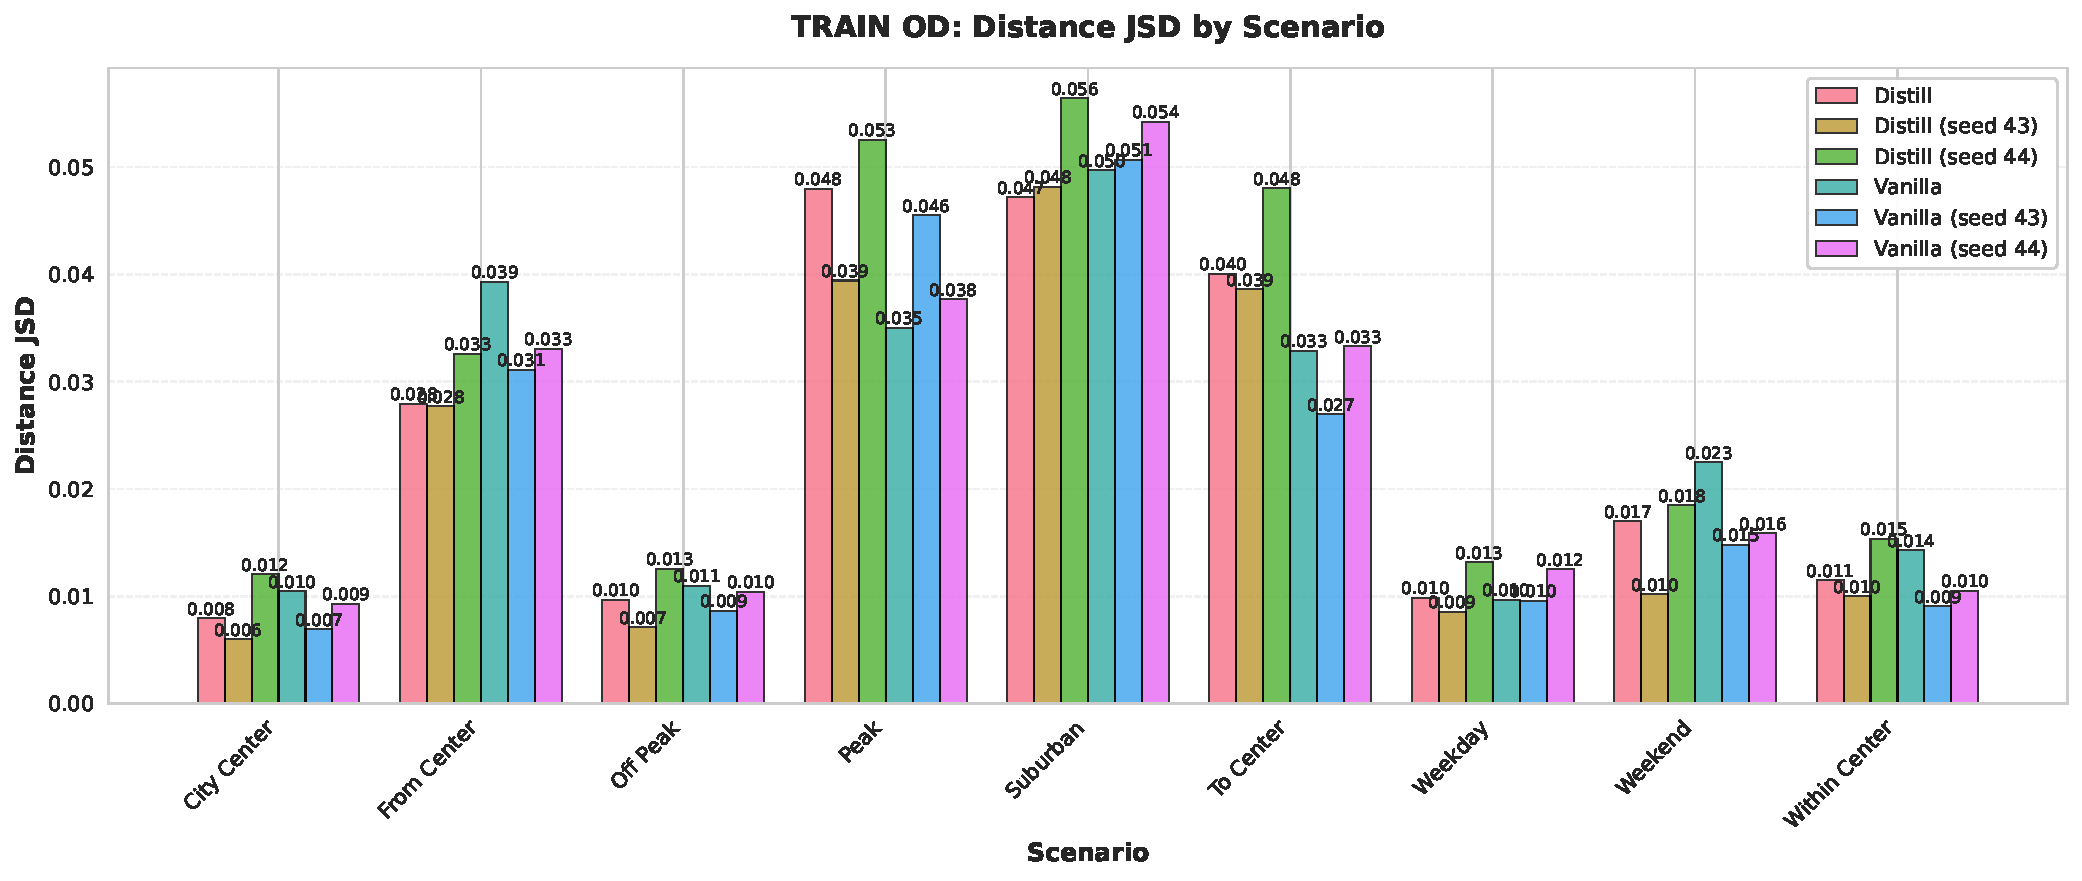
\includegraphics[width=\linewidth]{assets/plots/eval/porto/scenarios/train_od_scenario_comparison.pdf}
        \caption{Train OD scenarios}
    \end{subfigure}
    \begin{subfigure}{0.49\linewidth}
        \centering
        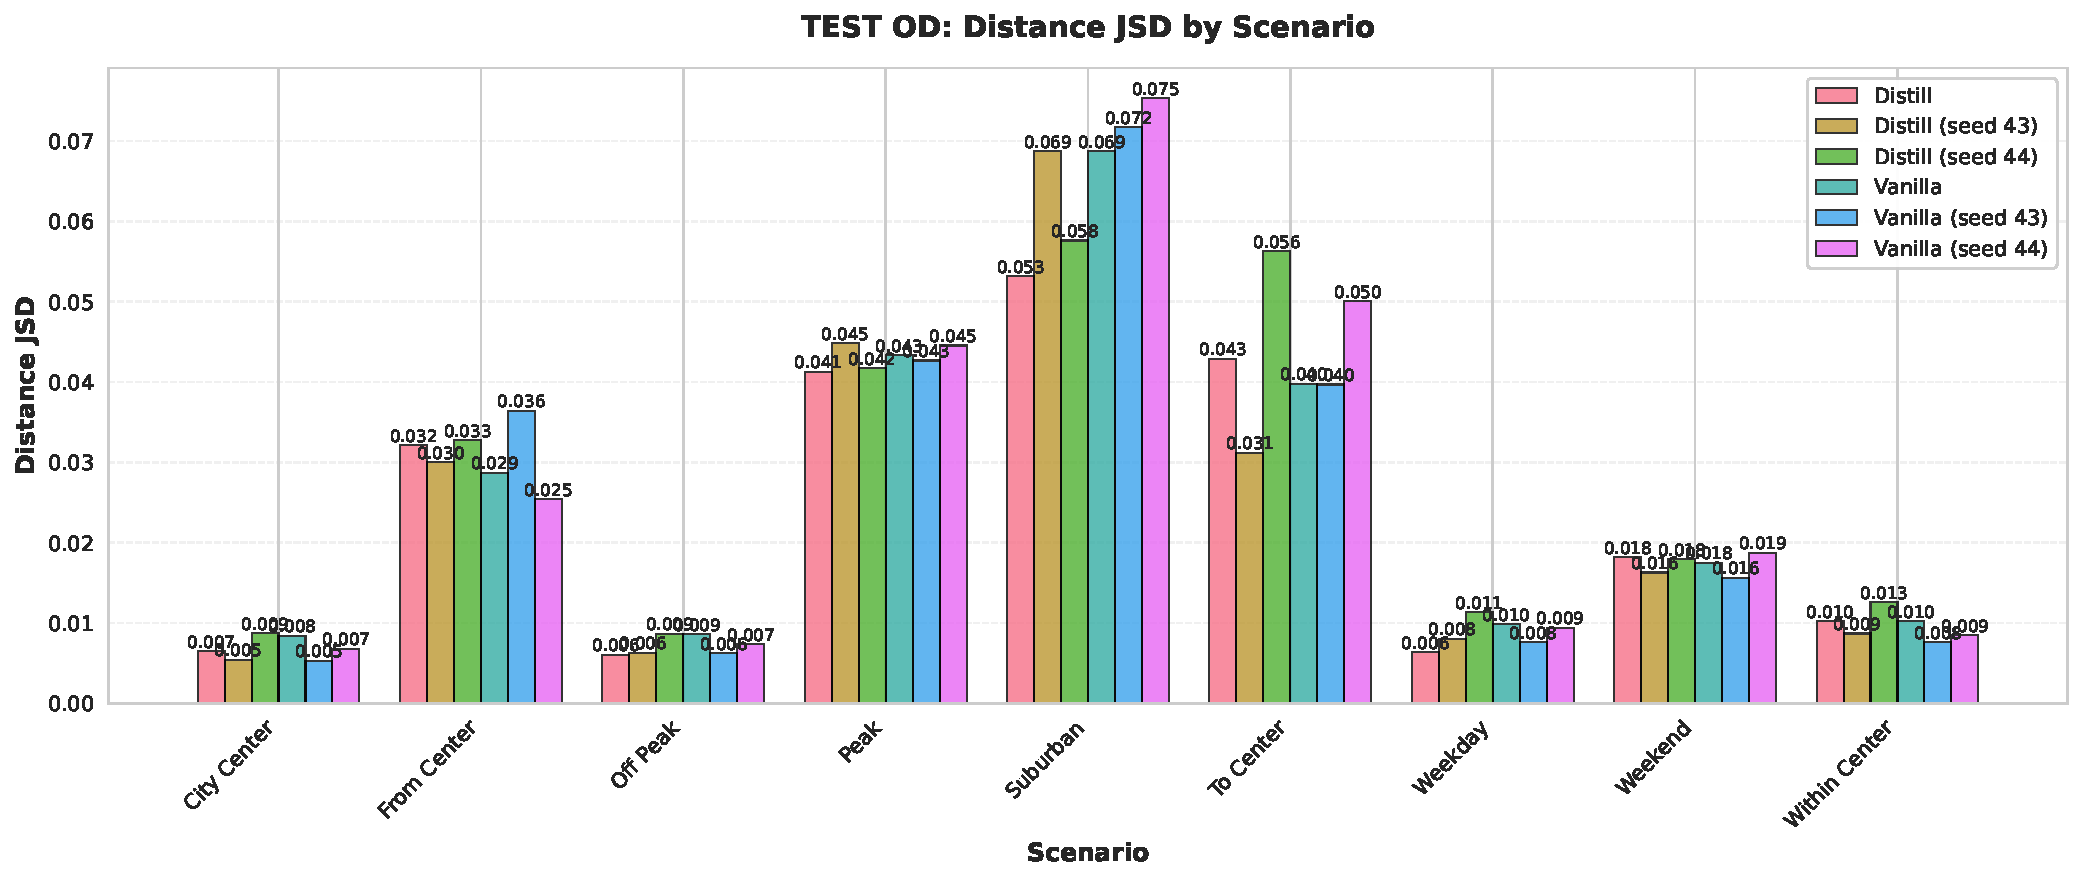
\includegraphics[width=\linewidth]{assets/plots/eval/porto/scenarios/test_od_scenario_comparison.pdf}
        \caption{Test OD scenarios}
    \end{subfigure}
    \caption{Porto scenario comparison across train and test OD pairs. Performance varies by spatial context, with stronger improvements in less urbanized areas.}
    \label{fig:appendix-porto-scenario-comparison}
\end{figure}

\begin{figure}[H]
    \centering
    \begin{subfigure}{0.49\linewidth}
        \centering
        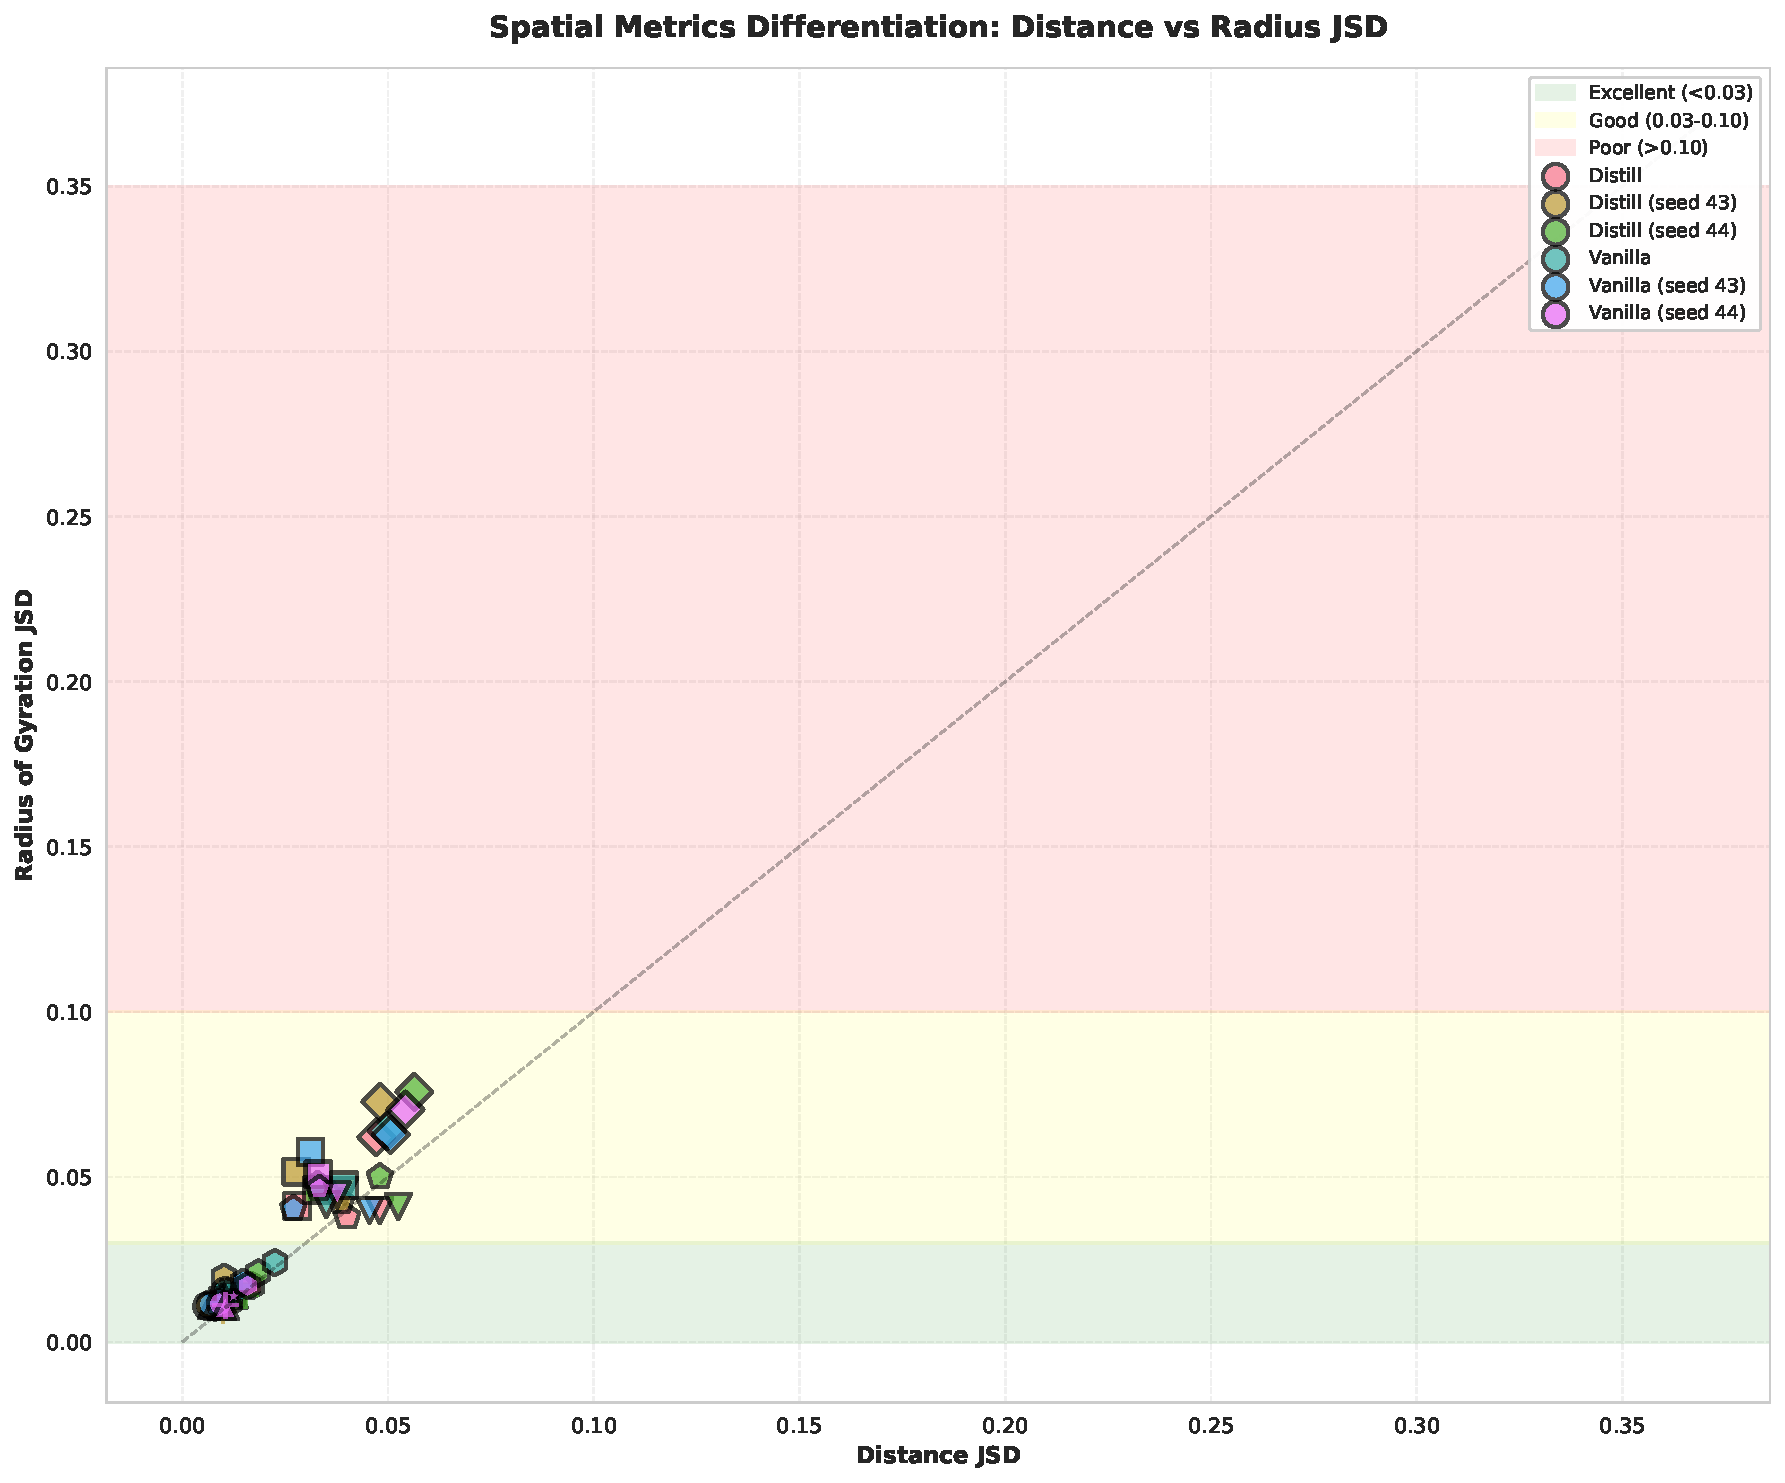
\includegraphics[width=\linewidth]{assets/plots/eval/porto/scenarios/spatial_metrics_differentiation.pdf}
        \caption{Spatial differentiation}
    \end{subfigure}
    \begin{subfigure}{0.49\linewidth}
        \centering
        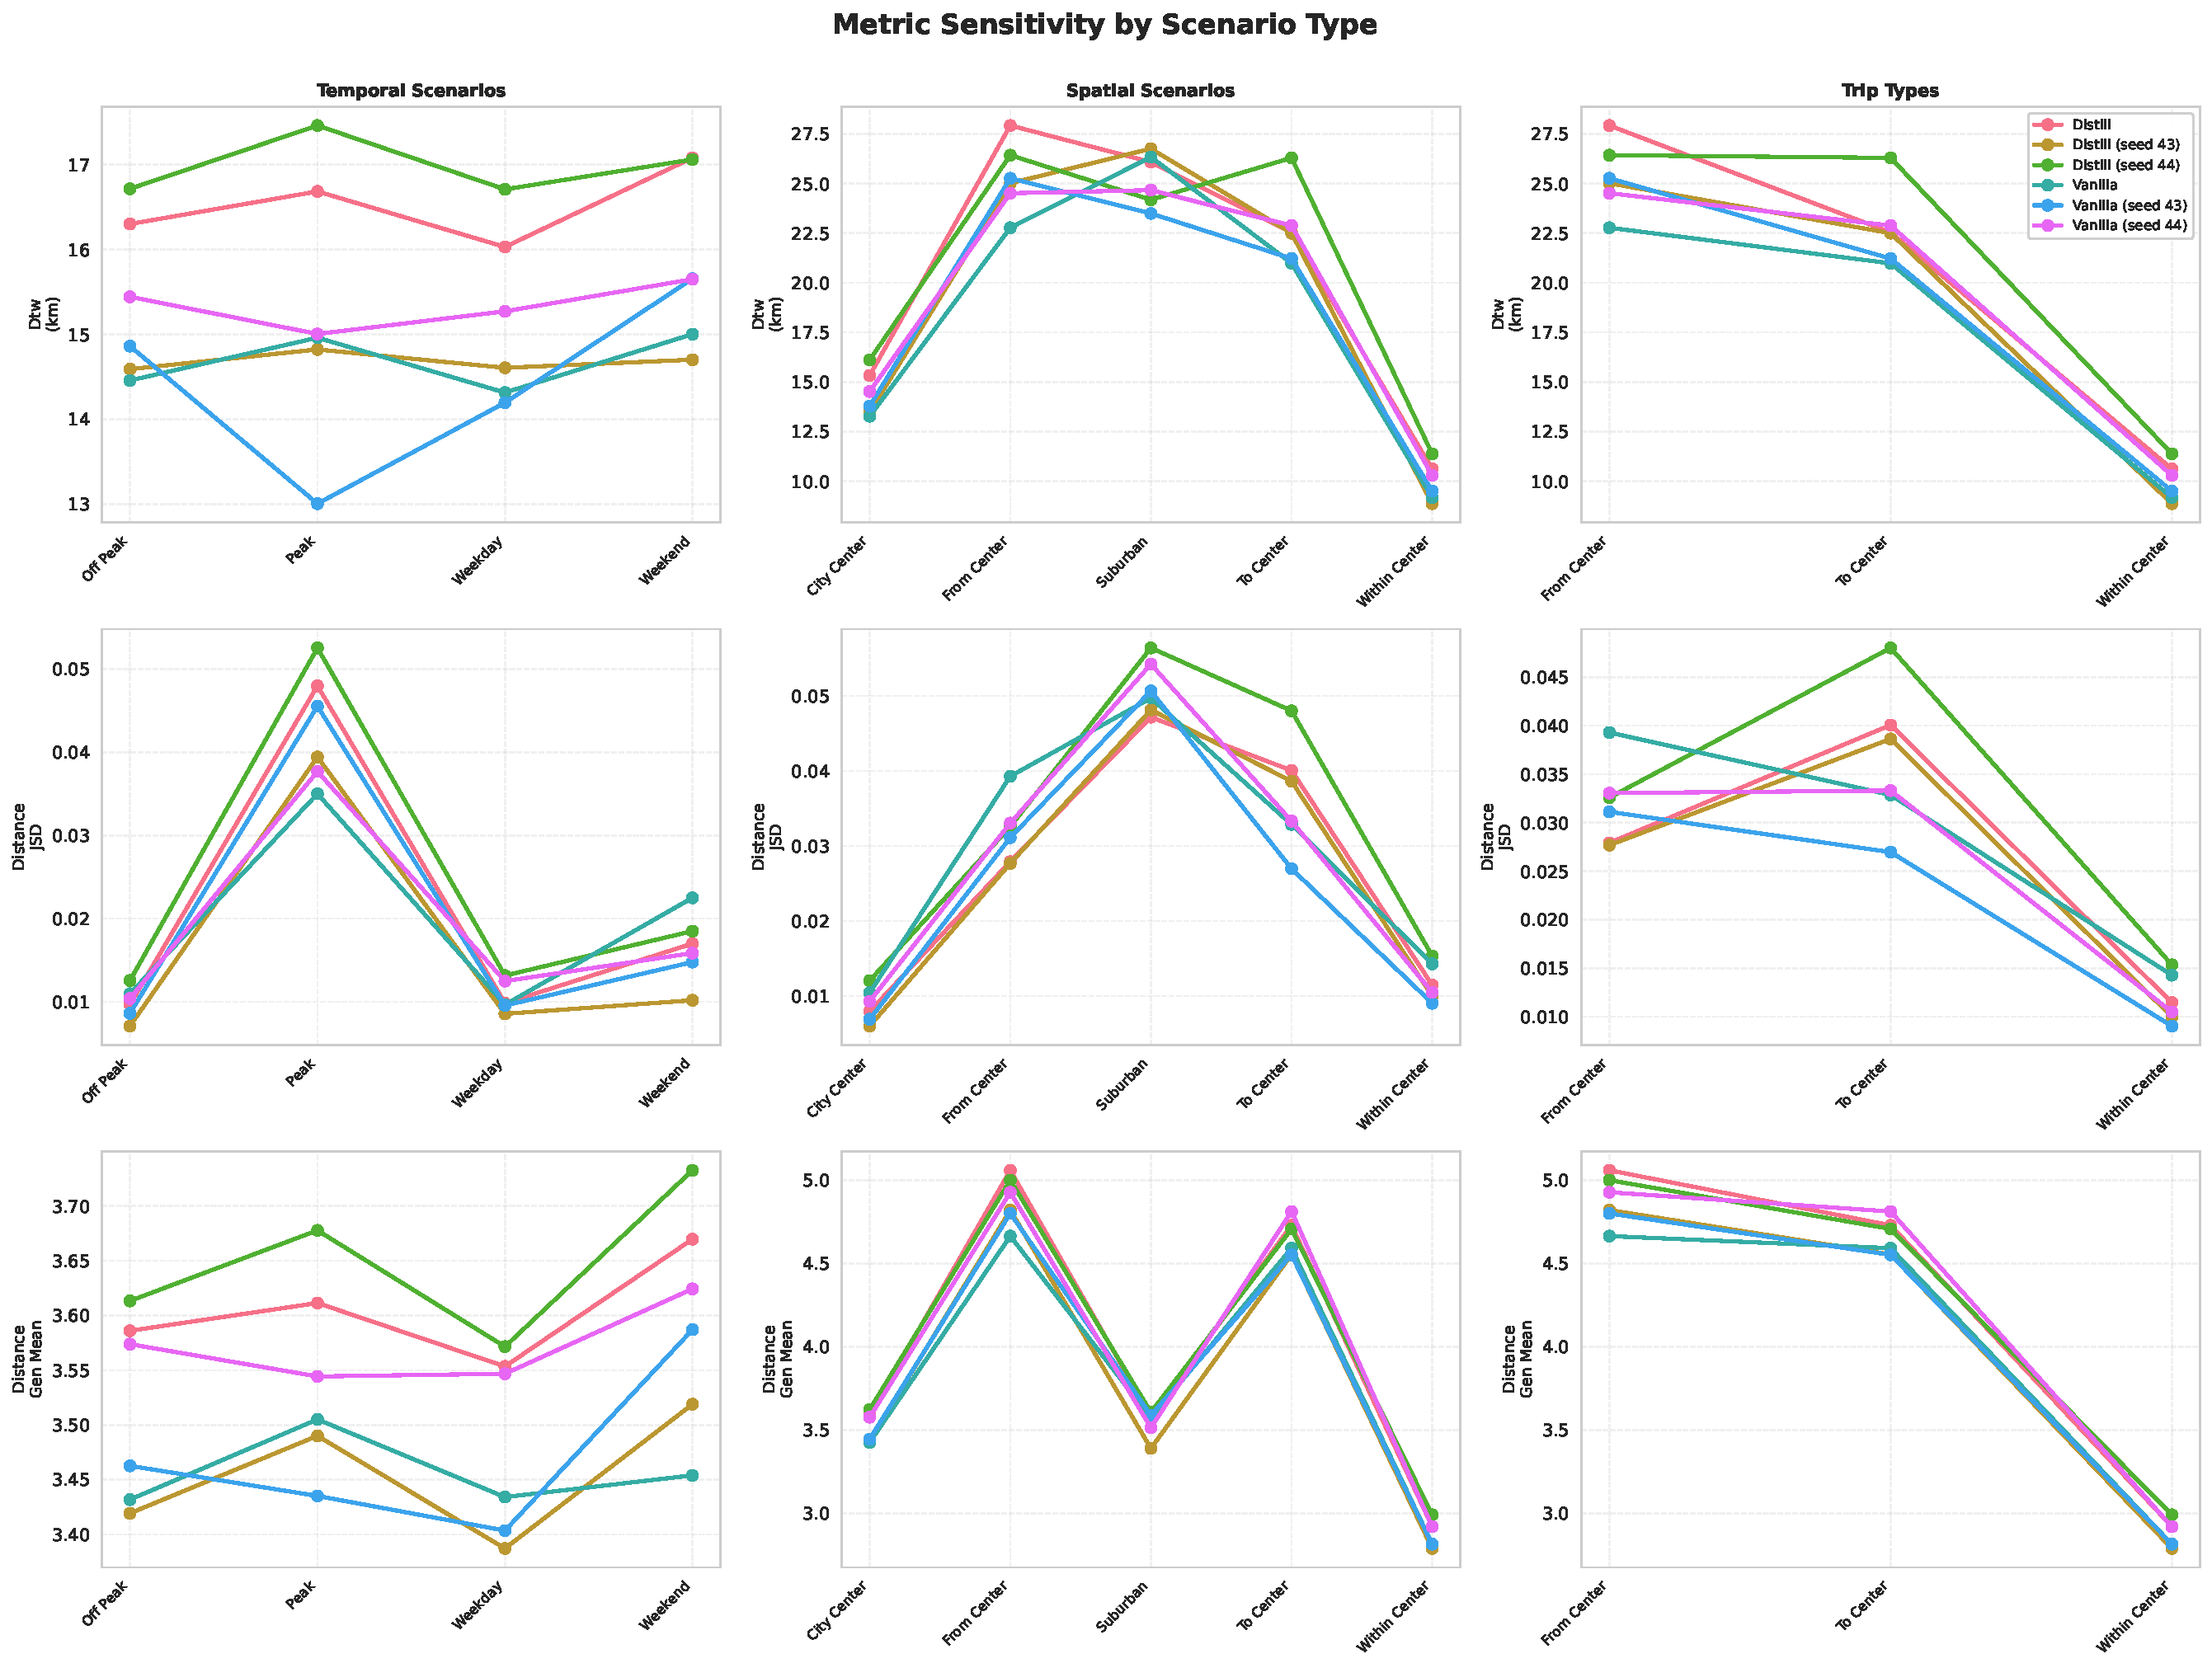
\includegraphics[width=\linewidth]{assets/plots/eval/porto/scenarios/metric_sensitivity_by_scenario.pdf}
        \caption{Metric sensitivity}
    \end{subfigure}
    \caption{Porto spatial context differentiation and metric sensitivity by scenario. Different metrics respond differently to distillation across contexts.}
    \label{fig:appendix-porto-scenario-sensitivity}
\end{figure}

\subsubsection{Trajectory Examples (Beijing)}
\label{app:traj-beijing}

Figures~\ref{fig:appendix-beijing-traj-train} and~\ref{fig:appendix-beijing-traj-test} show representative trajectory comparisons for Beijing train and test OD pairs, illustrating the qualitative differences between vanilla and distilled model generations.

\begin{figure}[H]
    \centering
    \begin{subfigure}{0.49\linewidth}
        \centering
        \includegraphics[width=\linewidth]{assets/plots/eval/beijing/trajectories/train_od_comparison_1_origin32347_dest26801.pdf}
        \caption{Train OD 1}
    \end{subfigure}
    \begin{subfigure}{0.49\linewidth}
        \centering
        \includegraphics[width=\linewidth]{assets/plots/eval/beijing/trajectories/train_od_comparison_3_origin32347_dest37646.pdf}
        \caption{Train OD 3}
    \end{subfigure}
    \begin{subfigure}{0.49\linewidth}
        \centering
        \includegraphics[width=\linewidth]{assets/plots/eval/beijing/trajectories/train_od_comparison_5_origin2466_dest8733.pdf}
        \caption{Train OD 5}
    \end{subfigure}
    \begin{subfigure}{0.49\linewidth}
        \centering
        \includegraphics[width=\linewidth]{assets/plots/eval/beijing/trajectories/train_od_comparison_7_origin20252_dest22542.pdf}
        \caption{Train OD 7}
    \end{subfigure}
    \caption{Beijing train OD trajectory examples. Distilled models generate complete paths reaching destinations, while vanilla models frequently terminate prematurely.}
    \label{fig:appendix-beijing-traj-train}
\end{figure}

\begin{figure}[H]
    \centering
    \begin{subfigure}{0.49\linewidth}
        \centering
        \includegraphics[width=\linewidth]{assets/plots/eval/beijing/trajectories/test_od_comparison_1_origin4462_dest35846.pdf}
        \caption{Test OD 1}
    \end{subfigure}
    \begin{subfigure}{0.49\linewidth}
        \centering
        \includegraphics[width=\linewidth]{assets/plots/eval/beijing/trajectories/test_od_comparison_3_origin24387_dest15499.pdf}
        \caption{Test OD 3}
    \end{subfigure}
    \begin{subfigure}{0.49\linewidth}
        \centering
        \includegraphics[width=\linewidth]{assets/plots/eval/beijing/trajectories/test_od_comparison_5_origin36493_dest3549.pdf}
        \caption{Test OD 5}
    \end{subfigure}
    \begin{subfigure}{0.49\linewidth}
        \centering
        \includegraphics[width=\linewidth]{assets/plots/eval/beijing/trajectories/test_od_comparison_7_origin27117_dest12017.pdf}
        \caption{Test OD 7}
    \end{subfigure}
    \caption{Beijing test OD trajectory examples. Generalization to unseen OD pairs demonstrates robust spatial understanding transferred from teacher.}
    \label{fig:appendix-beijing-traj-test}
\end{figure}

\subsubsection{Trajectory Examples (Porto)}
\label{app:traj-porto}

Figures~\ref{fig:appendix-porto-traj-train} and~\ref{fig:appendix-porto-traj-test} show representative trajectory comparisons for Porto train and test OD pairs, illustrating context-dependent performance patterns.

\begin{figure}[H]
    \centering
    \begin{subfigure}{0.49\linewidth}
        \centering
        \includegraphics[width=\linewidth]{assets/plots/eval/porto/trajectories/train_od_comparison_1_origin8237_dest1036.pdf}
        \caption{Train OD 1}
    \end{subfigure}
    \begin{subfigure}{0.49\linewidth}
        \centering
        \includegraphics[width=\linewidth]{assets/plots/eval/porto/trajectories/train_od_comparison_3_origin7840_dest3067.pdf}
        \caption{Train OD 3}
    \end{subfigure}
    \begin{subfigure}{0.49\linewidth}
        \centering
        \includegraphics[width=\linewidth]{assets/plots/eval/porto/trajectories/train_od_comparison_5_origin320_dest8550.pdf}
        \caption{Train OD 5}
    \end{subfigure}
    \begin{subfigure}{0.49\linewidth}
        \centering
        \includegraphics[width=\linewidth]{assets/plots/eval/porto/trajectories/train_od_comparison_7_origin712_dest8443.pdf}
        \caption{Train OD 7}
    \end{subfigure}
    \caption{Porto train OD trajectory examples. Both vanilla and distilled models achieve high path completion rates, with subtle differences in route selection.}
    \label{fig:appendix-porto-traj-train}
\end{figure}

\begin{figure}[H]
    \centering
    \begin{subfigure}{0.49\linewidth}
        \centering
        \includegraphics[width=\linewidth]{assets/plots/eval/porto/trajectories/test_od_comparison_1_origin9991_dest542.pdf}
        \caption{Test OD 1}
    \end{subfigure}
    \begin{subfigure}{0.49\linewidth}
        \centering
        \includegraphics[width=\linewidth]{assets/plots/eval/porto/trajectories/test_od_comparison_3_origin587_dest554.pdf}
        \caption{Test OD 3}
    \end{subfigure}
    \begin{subfigure}{0.49\linewidth}
        \centering
        \includegraphics[width=\linewidth]{assets/plots/eval/porto/trajectories/test_od_comparison_5_origin5462_dest1997.pdf}
        \caption{Test OD 5}
    \end{subfigure}
    \begin{subfigure}{0.49\linewidth}
        \centering
        \includegraphics[width=\linewidth]{assets/plots/eval/porto/trajectories/test_od_comparison_7_origin3067_dest899.pdf}
        \caption{Test OD 7}
    \end{subfigure}
    \caption{Porto test OD trajectory examples. Performance on held-out OD pairs demonstrates generalization to new spatial contexts.}
    \label{fig:appendix-porto-traj-test}
\end{figure}

\subsubsection{Cross-Model Trajectory Comparisons (Beijing)}
\label{app:cross-model-beijing}

Figures~\ref{fig:appendix-beijing-cross-test} and~\ref{fig:appendix-beijing-cross-train} present direct side-by-side trajectory visualizations comparing vanilla and distilled model outputs for Beijing, providing qualitative evidence of improved path completion.

\begin{figure}[H]
    \centering
    \begin{subfigure}{0.49\linewidth}
        \centering
        \includegraphics[width=\linewidth]{assets/plots/eval/beijing/cross_model/test_od_comparison_1_origin4462_dest35846.pdf}
        \caption{Test OD 1}
    \end{subfigure}
    \begin{subfigure}{0.49\linewidth}
        \centering
        \includegraphics[width=\linewidth]{assets/plots/eval/beijing/cross_model/test_od_comparison_3_origin24387_dest15499.pdf}
        \caption{Test OD 3}
    \end{subfigure}
    \begin{subfigure}{0.49\linewidth}
        \centering
        \includegraphics[width=\linewidth]{assets/plots/eval/beijing/cross_model/test_od_comparison_5_origin36493_dest3549.pdf}
        \caption{Test OD 5}
    \end{subfigure}
    \begin{subfigure}{0.49\linewidth}
        \centering
        \includegraphics[width=\linewidth]{assets/plots/eval/beijing/cross_model/test_od_comparison_7_origin27117_dest12017.pdf}
        \caption{Test OD 7}
    \end{subfigure}
    \caption{Beijing test OD cross-model comparisons showing vanilla (premature termination) vs distilled (complete paths) behavior.}
    \label{fig:appendix-beijing-cross-test}
\end{figure}

\begin{figure}[H]
    \centering
    \begin{subfigure}{0.49\linewidth}
        \centering
        \includegraphics[width=\linewidth]{assets/plots/eval/beijing/cross_model/train_od_comparison_1_origin32347_dest26801.pdf}
        \caption{Train OD 1}
    \end{subfigure}
    \begin{subfigure}{0.49\linewidth}
        \centering
        \includegraphics[width=\linewidth]{assets/plots/eval/beijing/cross_model/train_od_comparison_3_origin32347_dest37646.pdf}
        \caption{Train OD 3}
    \end{subfigure}
    \begin{subfigure}{0.49\linewidth}
        \centering
        \includegraphics[width=\linewidth]{assets/plots/eval/beijing/cross_model/train_od_comparison_5_origin2466_dest8733.pdf}
        \caption{Train OD 5}
    \end{subfigure}
    \begin{subfigure}{0.49\linewidth}
        \centering
        \includegraphics[width=\linewidth]{assets/plots/eval/beijing/cross_model/train_od_comparison_7_origin20252_dest22542.pdf}
        \caption{Train OD 7}
    \end{subfigure}
    \caption{Beijing train OD cross-model comparisons demonstrating consistent distillation improvements even on training set OD pairs.}
    \label{fig:appendix-beijing-cross-train}
\end{figure}

\subsubsection{Cross-Model Trajectory Comparisons (Porto)}
\label{app:cross-model-porto}

Figures~\ref{fig:appendix-porto-cross-test} through~\ref{fig:appendix-porto-scenario-suburban} present direct side-by-side trajectory visualizations for Porto, showing subtle differences in route selection and distribution quality. Additionally, Figures~\ref{fig:appendix-porto-scenario-city-center} and~\ref{fig:appendix-porto-scenario-suburban} show scenario-specific comparisons revealing context-dependent performance patterns.

\begin{figure}[H]
    \centering
    \begin{subfigure}{0.49\linewidth}
        \centering
        \includegraphics[width=\linewidth]{assets/plots/eval/porto/cross_model/test/test_od_comparison_1_origin9991_dest542.pdf}
        \caption{Test OD 1}
    \end{subfigure}
    \begin{subfigure}{0.49\linewidth}
        \centering
        \includegraphics[width=\linewidth]{assets/plots/eval/porto/cross_model/test/test_od_comparison_3_origin587_dest554.pdf}
        \caption{Test OD 3}
    \end{subfigure}
    \begin{subfigure}{0.49\linewidth}
        \centering
        \includegraphics[width=\linewidth]{assets/plots/eval/porto/cross_model/test/test_od_comparison_5_origin5462_dest1997.pdf}
        \caption{Test OD 5}
    \end{subfigure}
    \begin{subfigure}{0.49\linewidth}
        \centering
        \includegraphics[width=\linewidth]{assets/plots/eval/porto/cross_model/test/test_od_comparison_7_origin3067_dest899.pdf}
        \caption{Test OD 7}
    \end{subfigure}
    \caption{Porto test OD cross-model comparisons. Both models complete most paths; differences appear in route choice and spatial distribution.}
    \label{fig:appendix-porto-cross-test}
\end{figure}

\begin{figure}[H]
    \centering
    \begin{subfigure}{0.49\linewidth}
        \centering
        \includegraphics[width=\linewidth]{assets/plots/eval/porto/cross_model/train/train_od_comparison_1_origin8237_dest1036.pdf}
        \caption{Train OD 1}
    \end{subfigure}
    \begin{subfigure}{0.49\linewidth}
        \centering
        \includegraphics[width=\linewidth]{assets/plots/eval/porto/cross_model/train/train_od_comparison_3_origin7840_dest3067.pdf}
        \caption{Train OD 3}
    \end{subfigure}
    \begin{subfigure}{0.49\linewidth}
        \centering
        \includegraphics[width=\linewidth]{assets/plots/eval/porto/cross_model/train/train_od_comparison_5_origin320_dest8550.pdf}
        \caption{Train OD 5}
    \end{subfigure}
    \begin{subfigure}{0.49\linewidth}
        \centering
        \includegraphics[width=\linewidth]{assets/plots/eval/porto/cross_model/train/train_od_comparison_7_origin712_dest8443.pdf}
        \caption{Train OD 7}
    \end{subfigure}
    \caption{Porto train OD cross-model comparisons showing baseline high performance with marginal distillation improvements.}
    \label{fig:appendix-porto-cross-train}
\end{figure}

\paragraph{Scenario-Specific Cross-Model Comparisons (Porto)}

Figures~\ref{fig:appendix-porto-scenario-city-center} and~\ref{fig:appendix-porto-scenario-suburban} present cross-model trajectory comparisons for specific spatial scenarios, demonstrating how distillation benefits vary by urban context. City center trajectories show where teacher knowledge provides spatial guidance, while suburban trajectories reveal contexts where vanilla models already perform well.

\begin{figure}[H]
    \centering
    \begin{subfigure}{0.49\linewidth}
        \centering
        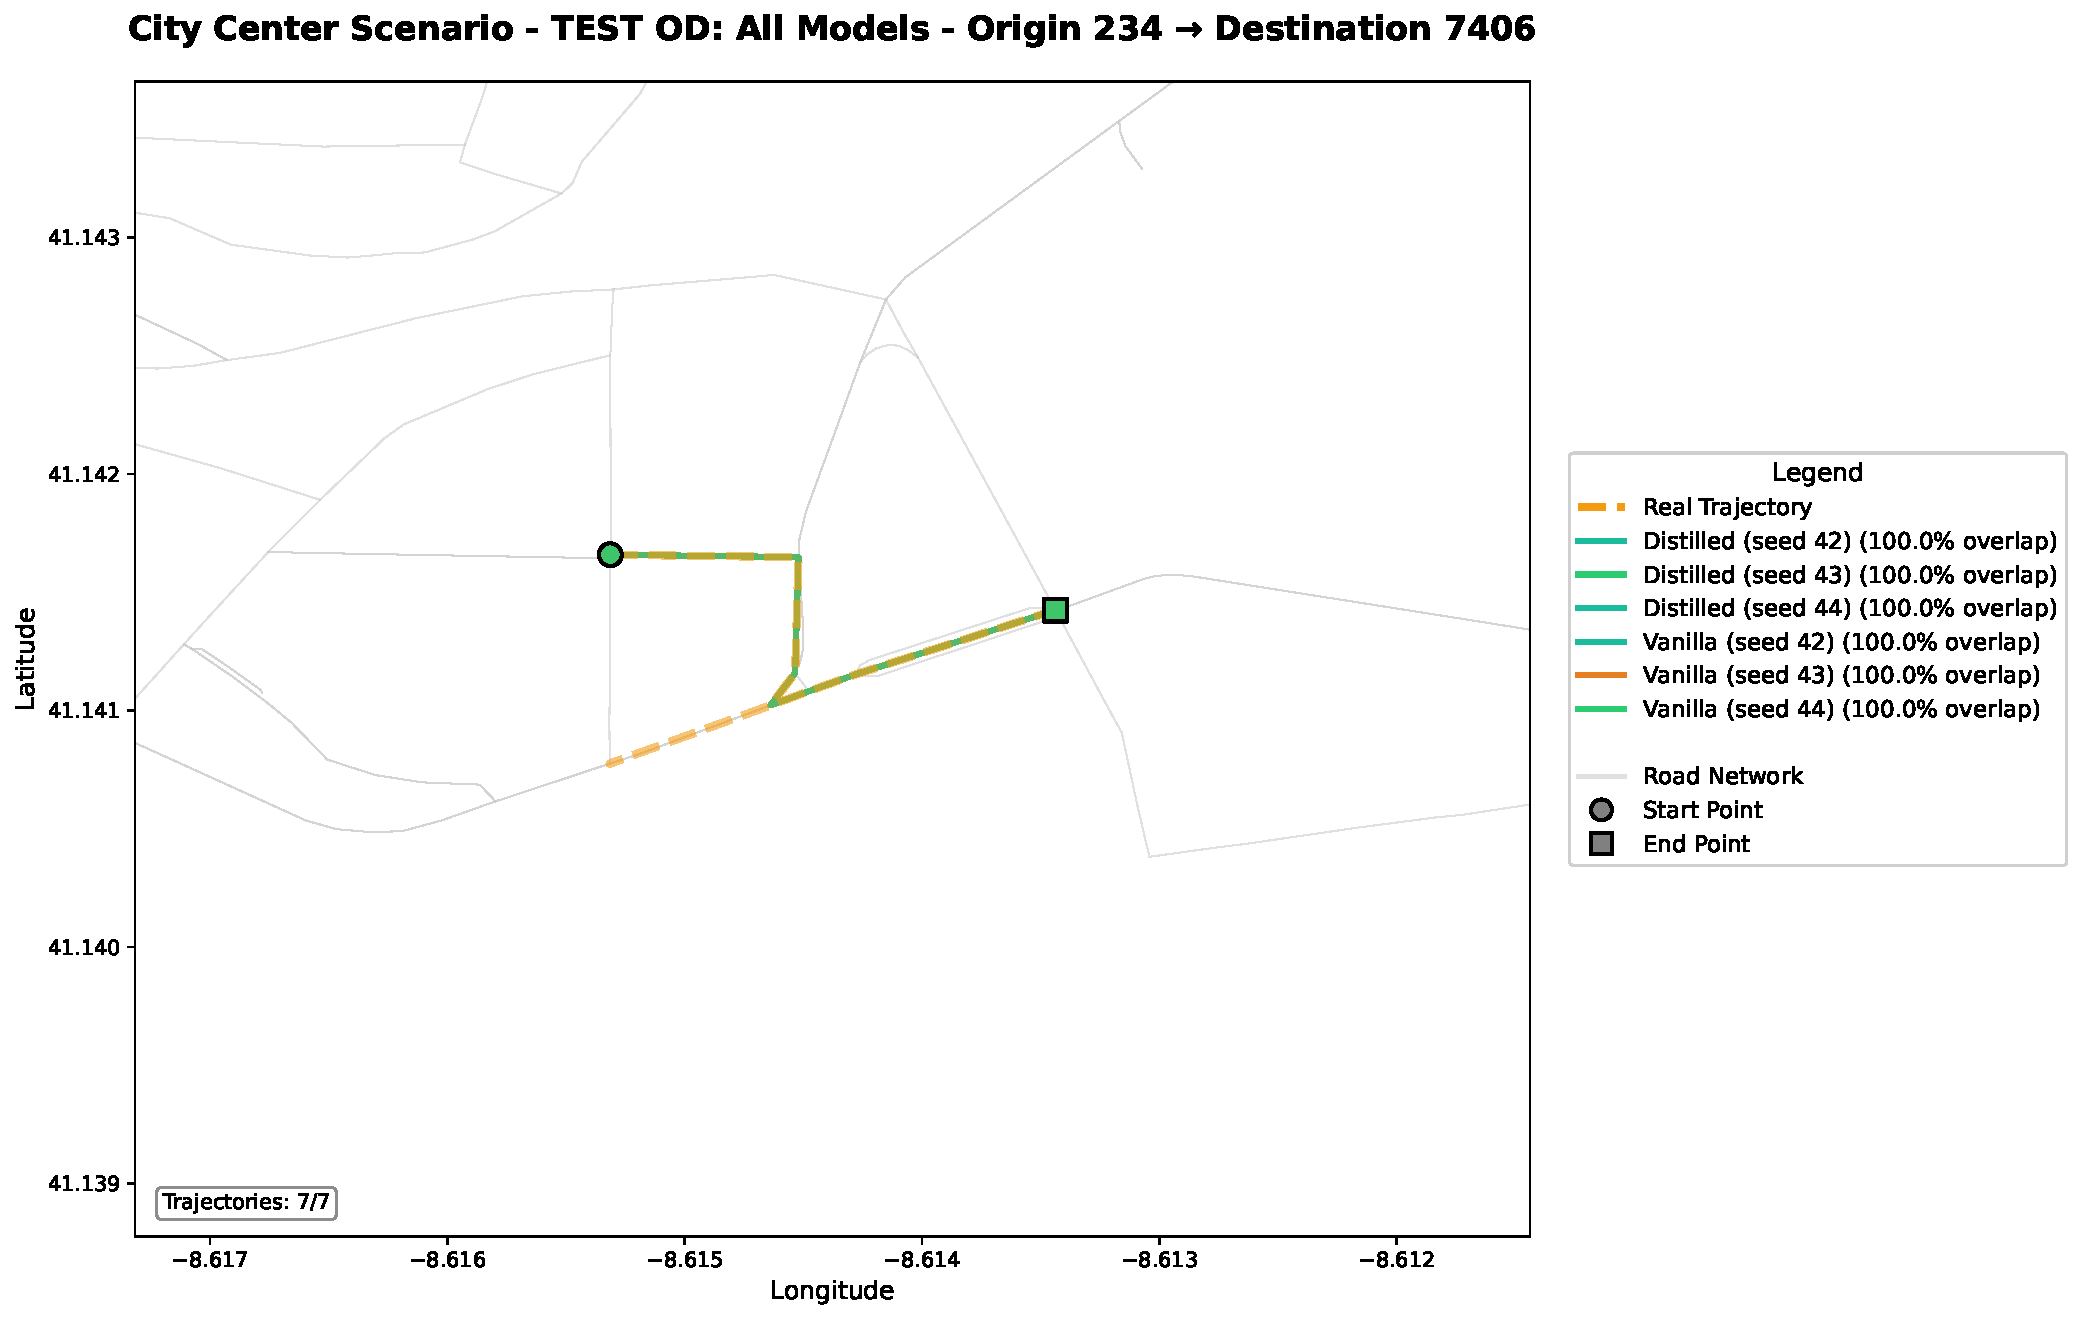
\includegraphics[width=\linewidth]{assets/plots/eval/porto/scenario_cross_model/test/city_center/test_od_comparison_1_origin234_dest7406.pdf}
        \caption{City center: Test OD 1}
    \end{subfigure}
    \begin{subfigure}{0.49\linewidth}
        \centering
        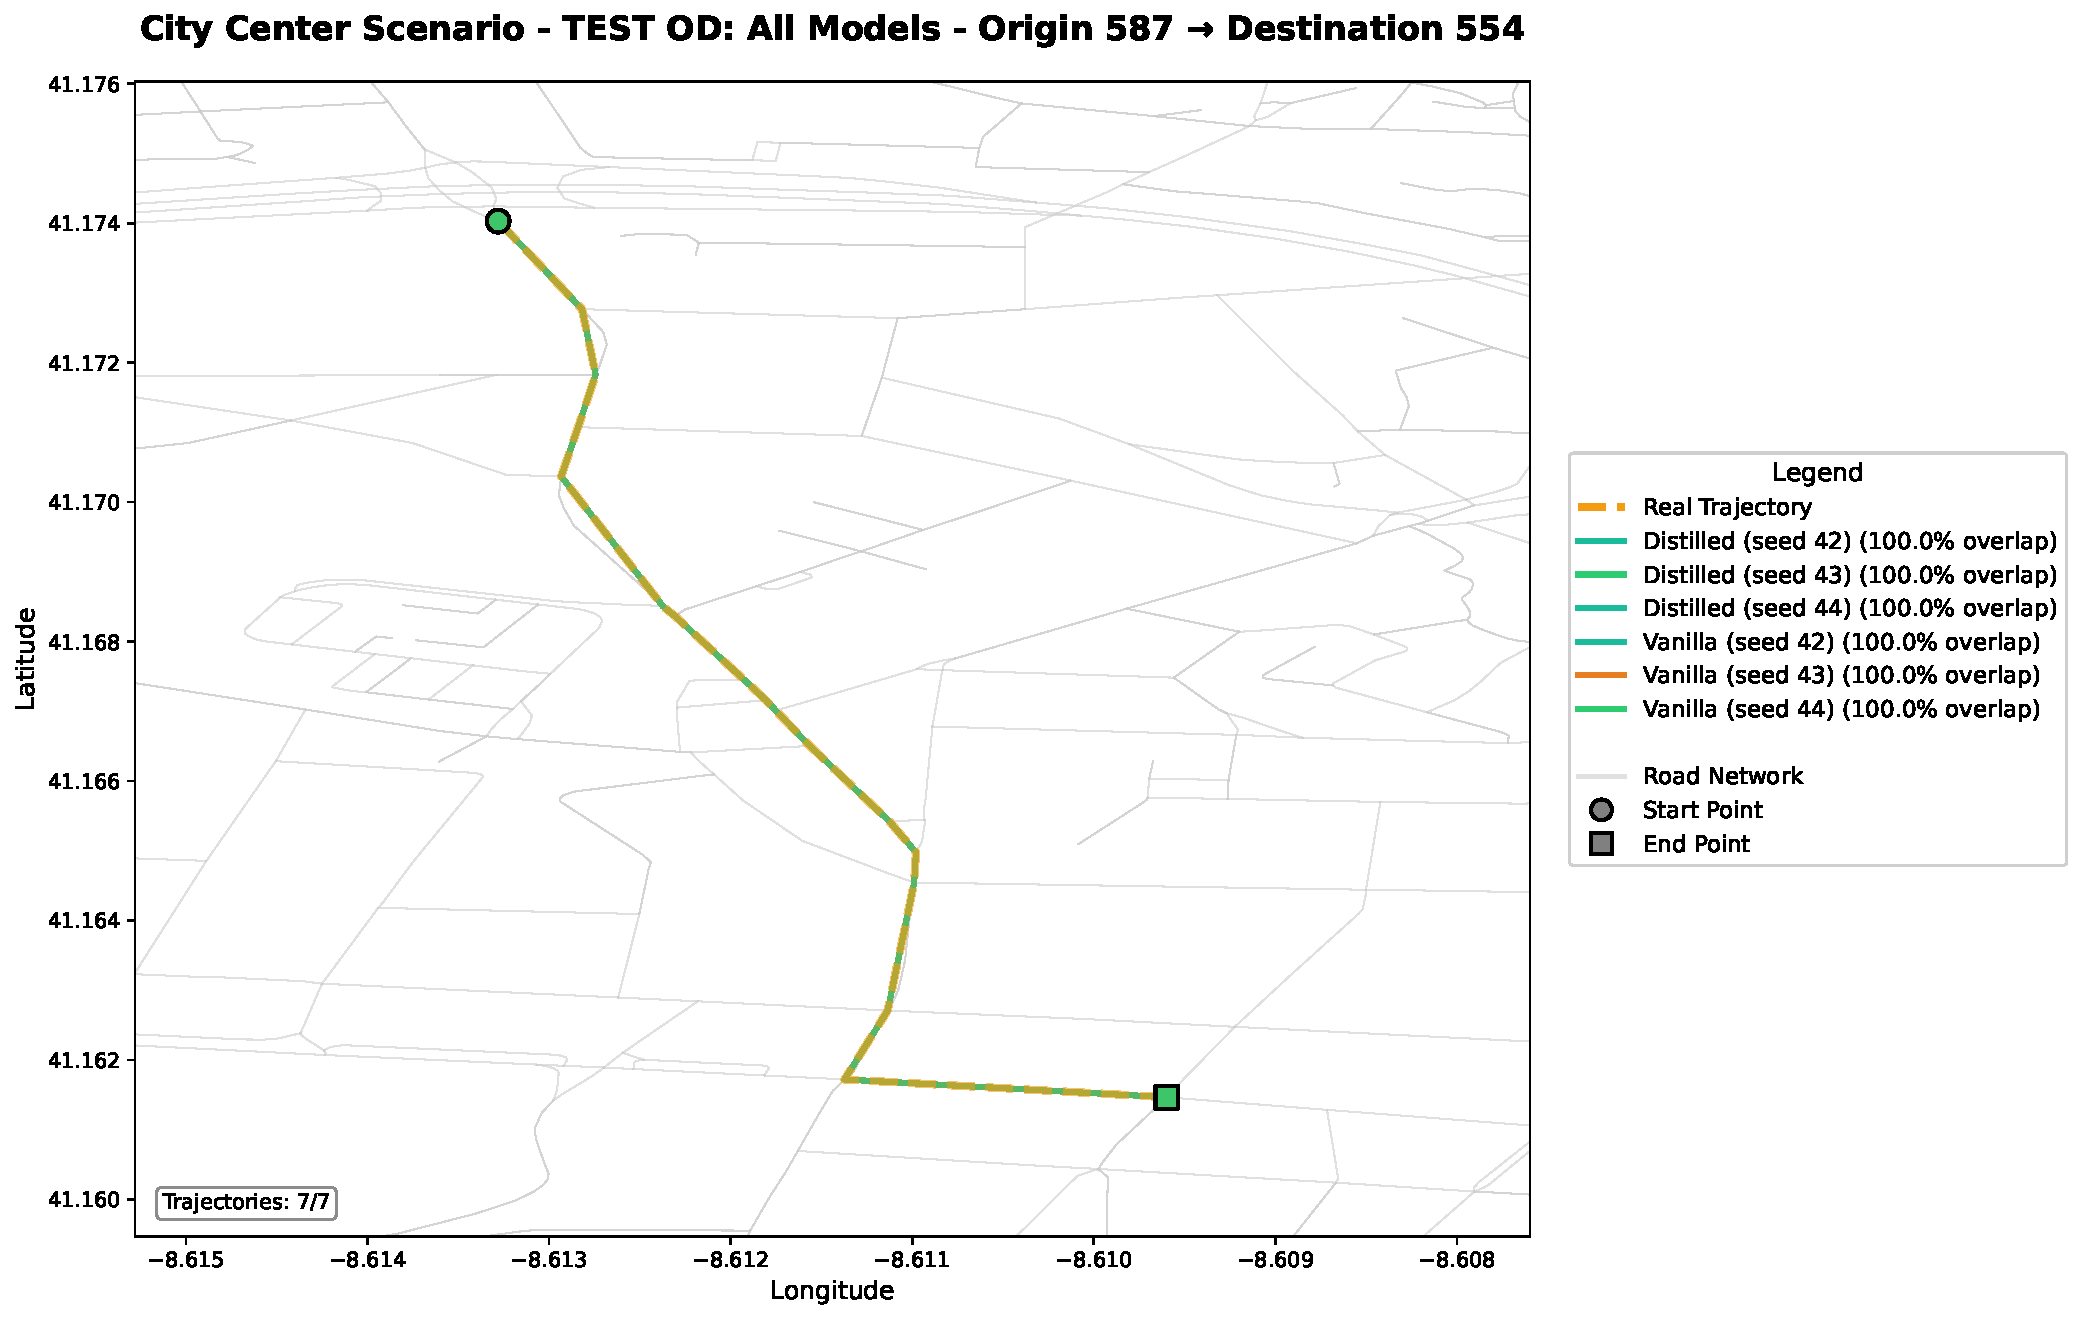
\includegraphics[width=\linewidth]{assets/plots/eval/porto/scenario_cross_model/test/city_center/test_od_comparison_3_origin587_dest554.pdf}
        \caption{City center: Test OD 3}
    \end{subfigure}
    \begin{subfigure}{0.49\linewidth}
        \centering
        \includegraphics[width=\linewidth]{assets/plots/eval/porto/scenario_cross_model/train/city_center/train_od_comparison_1_origin8435_dest357.pdf}
        \caption{City center: Train OD 1}
    \end{subfigure}
    \begin{subfigure}{0.49\linewidth}
        \centering
        \includegraphics[width=\linewidth]{assets/plots/eval/porto/scenario_cross_model/train/city_center/train_od_comparison_3_origin10016_dest1949.pdf}
        \caption{City center: Train OD 3}
    \end{subfigure}
    \caption{Porto city center scenario cross-model comparisons. Dense urban context where distillation provides spatial guidance benefits, reflecting teacher (LM-TAD) training domain expertise.}
    \label{fig:appendix-porto-scenario-city-center}
\end{figure}

\begin{figure}[H]
    \centering
    \begin{subfigure}{0.8\linewidth}
        \centering
        \includegraphics[width=\linewidth]{assets/plots/eval/porto/scenario_cross_model/test/suburban/test_od_comparison_1_origin10232_dest2811.pdf}
        \caption{Suburban: Test OD comparison (only one suitable pair found for this scenario)}
    \end{subfigure}
    \caption{Porto suburban scenario cross-model comparison. Lower-density context where vanilla already performs well, showing limited marginal benefit from distillation. Demonstrates spatial localization of teacher knowledge.}
    \label{fig:appendix-porto-scenario-suburban}
\end{figure}
